% ============================================================
%  第五卷 第十三章 晶体的对称性（§128–§141）
%  底本：高教社中文版第5版（束仁贵/束莼 译，郑伟谋 校）
%  本章插图 5 幅（图55–图59，均在 §130）；无习题（与原书一致）；
%  表格：§130 晶系参数数目表、§131 晶类表、§132 表1、§134 表2/表3、
%  §135 C2 特征标小表，均按原书 p-370…p-384 用 tabular 重排。
%  正文圈码 46 处（①×26、②×11、③×6、④×2、⑤×1）已全部还原为 \footnote，
%  并按 pages300 页面逐页转录脚注文本（页面分布：p366①、p367①、p374①、p375①、
%  p376①、p377①、p378①、p379①②③、p380①、p381①②③④、p383①、p384①、p385①、
%  p386①②、p387①②、p388①②③④⑤、p389①②③、p390①、p391①②③、p392①、
%  p393①②、p394①②、p395①、p397①②③、p398①、p399①②；无脚注页：
%  p368–p373、p382、p396）。
%  已修正的 OCR/原书错误（均对照 原书转换/pages/p-366…p-400.png 核实）：
%   1. OCR 目录"晶体的対称性"之"対"系日文汉字，按正文改为"对"。
%   2. §128 行14263 "函数 ρ^𝕆"→"函数 ρ①"；行14267 "ρ(x,y,z))1还具有"
%      之伪"1"删除（p-366 无此字符）。
%   3. §129 行14293 a1,a2,a3 后伪逗号删；"行列式 β_ik 等于行列式 α_ik
%      的倒数"按原书 p-368 补绝对值：|β_ik|、|α_ik|。
%   4. §130 行14333 "设1(图55)"→"设 A（图55）"（p-369 印 A）；
%      Γ_′→Γ_t、Γ_s→Γ_q、Γ_e→Γ_c、C_δ→C_6（p-370/371）；
%      行14422 "如果图58所示的方式"原书即无"按"字，照排（见遗留）。
%   5. §131 晶类表按 p-374 重排：单斜行 C_s（OCR "c,"）、四方行 D_4
%      （OCR D_𝓼）、三方行 C_3（OCR c_*）等全部复原。
%   6. §132 "E.C.Φeopo"→Е.С.Федоров（p-375）；表1 按原书重排（OCR
%      类名 D_ι、D_⟪h、c_δ、o_b 等乱码复原）；"彼·此重合"→"彼此重合"。
%   7. §133 (133.5) 花括号内 "ℏ↓∥𝔻" 乱码按原书为"如果 i≠k / 如果 i=k"；
%      行14553 "b·r=♯♯χ" 按原书 p-377 为 "b·r=常数"、平面距原点
%      "常数/b"；行14569 "相交于…=点"→"三点"；行14531 "倒格基矢①4"
%      之伪"4"删。
%   8. §134 行14615 e^{i★·α}→e^{ik·a}；行14617 k′=Pk^{(1)}→k′=Pk①；
%      "小表⊥ⁿ"→"小表示"；行14633 "其中u。形成矢量k u_α 的点群表示
%      的基"→"其中 u_α 形成矢量 k 的点群表示的基"；行14637 "所组成的
%      数"→"所组成的群"（按文意）；行14658 表2 按 p-382 全部重排
%      （Γ₁：2,−2,2,−2,0,…；Γ₂：2,−2,−2,2,0,…）。
%   9. §135 行14705 "∝0^{-101}"→∝e^{-iωt}；"位移u，"→u_s；行14719
%      "(1 5-1/2 1 3-5 1)"→"（但 1/2 除外）"；C_2 特征标表按 p-384
%      重排（A:1,1；B:1,−1）；行14740 平移特征标补第三列 (E|a₃):
%      2cos2πϰ（OCR 脉落）；行14752 以下 λ→Λ（原书 p-385 用大写 Λ）；
%      行14755 两相同矢量 "(−ϰ,−Λ,1/2) 和 (−ϰ,−Λ,1/2)" 前者按文意改
%      为 (ϰ,Λ,1/2)（原书排印重影）；行14783 "χ_k[(P|k)]"→
%      "χ_k[(P|τ)]"（原书排印 (P|k)，按 (135.4) 应为 τ）；
%      行14809 "旋转元素Φ;n_k"→"旋转元素①；n_k"（该①即(135.5)后脚注，已按
%      p386① 归位转录）。
%  10. §136 行14863 O_h′→O_h^7；"(I|∇∇∇)"→(I|τ)；"F_{2g}+F_{2u}⊙"
%      之 ⊙→⑤（p-373 脚注号实为 5）；行14865 "k≡8k"→k=δk、
%      "Ĥ_𝔬"→Ĥ₀；行14867/14870 "D²{array}"→|D²|（原书 p-374 用竖线
%      记反对称直积：|D²|、|E²|、|F₁²|、|F₂²|）；行14888–14900 三个
%      分裂表按 p-375 补类头（E 2C₃ 3σ′／E C₂ 2C₄ 2σ 2σ′／E C₂′ σ σ′）。
%  11. §137 行14907 "J..朗道"→Л.Д.朗道（p-375）；行14930 以下
%      ΔF_∥、F_:、F_i、F_r、(ΔF_)_k 之下标乱码一律按原书为"总"
%      （ΔF_总，p-376 起）；行14946 (137.4)(137.5) 之 u_ik u*_ik 按
%      张量缩并指标及 (137.6) 改为 u_ik u*_lk，并补 OCR 丢失的 ⟨⟩；
%      "av=k′"乱码→"当 k′≠−k"；行14958 A_u→A_ll；行14965 绕γ轴→
%      绕y轴；行14988 (137.9) "dk_x(ϰ²)"→"dk_x d(ϰ²)"（按积分测度补 d）；
%      行14999 "平均涨落位φ移"→"平均涨落位移"；行15004 (137.11)
%      u_iu_i、A_ii→u_iu_l、A_il（p-378）。
%  12. §138 行15017 "设在晶格点的原子"→"设在晶格 r 点的原子"（p-378）；
%      行15029 θ′→b′、ρ_δ→ρ_b；行15052 χ_u→χ_il，且展开式指标按
%      p-379 为 (u_i1−u_i2)(u_l1−u_l2)=2⟨u_iu_l⟩−⟨u_i1u_l2⟩−⟨u_i2u_l1⟩
%      （OCR 末项下标误）；行15061 "在 k≳k_max ħck_max∼T 时"按原书
%      断句补逗号；行15072 α_b=b_i b_l Ā_il（OCR b_ib_i Ā_i）。
%  13. §139 行15093 C_*h,D_*,D_*→C_{∞h}、D_∞、D_{∞h}（p-380）；
%      "K_k 群"→K_h 群（p-381）。
%  14. §140 行15105 F_1→F_总；行15112 ∂n_t→∂n_l；行15124 首项
%      "[ρ(n·∇)n]²"之伪 ρ 删；行15139 "∇·n^②"→"∇·n②"；
%      行15177 "π/q₀ 这样的结构"句间补句号（p-383 分句）。
%  15. §141 χ_∘、χ_*、χ_0→χ_a（p-383/384）；行15208 (141.4)
%      "a₂(∇×ν)²_*"→a₂(∇×ν)_x²（p-384 印下标 x）；行15228 (141.6)
%      按 p-384 重排：⟨|ν_yk|²⟩（a₁k_y²…）、⟨|ν_xk|²⟩（a₂k_y²…）、
%      ⟨ν_ykν_xk⟩=0，并补 OCR 丢失的 ⟨⟩；行15236 (141.7) 补 ⟨⟩；
%      行15247 "∼ϰ*"→"∼ϰ⁴"；末段 ⟨ν_k²⟩∝1/φ(k_x,k_y)、⟨ν²⟩ 补 ⟨⟩。
%  遗留问题：
%   - 行14422（§130）"如果图58所示的方式用虚线联结"疑脱"按"字，
%     原书 p-372 同样如此，照排。
%   - 行14458（§131）"而使它变成正方形棱柱体"、行14991（§137）
%     "某点可大距离移动"、行14961"理所当然是"、行15077（§138）
%     "温度愈低速度愈慢"、行15095（§139）"彼此可自由的相对移动"、
%     行15185（§141）"n₀≡ñ"、行14705"偶数阶——2阶导数"均为原书
%     排印原文，照排。
%   - 表3（p-383）第三列类头 (C₂ˣ|0)(C₂ˣ|a₁) 与正文"C₂ 的轴沿 z 轴"
%     似不一致（原书如此），照排。
%   - §136 "群 T_d 的元素与 τ=(½½½) 下的反演 (I|τ) 结合得到"语序依
%     原书 p-373。
% ============================================================
\chapter{晶体的对称性}

\section{晶格的对称元素}

宏观物体最普遍的对称性在于物体中粒子位形的对称性.

运动着的原子和分子在物体中并不占据精确确定的位置，为了严格地统计描述它们的排布必须引入一个密度函数 $\rho(x,y,z)$ 来确定粒子在各个位置的概率：$\rho\,\mathrm{d}V$ 是单个粒子处于体积元 $\mathrm{d}V$ 内的概率.粒子位形的对称性质取决于使函数 $\rho(x,y,z)$ 保持不变的坐标变换（平移、转动、反映）.一个给定物体的所有这些对称变换的集合构成它的对称群.

如果物体由不同的原子构成，则函数 $\rho$ 必须对每一种原子单独确定.然而，这并不重要，因为在现实物体中所有这些函数实际上都具有相同的对称.同样地，我们也可以使用由所有原子在物体每一点产生的总电子密度所定义的函数 $\rho$\footnote{运动的电子不仅能产生平均电荷密度($e\rho$)，而且也产生平均电流密度$\boldsymbol{j}(x,y,z)$.电流非零的这种物体也具有“磁结构”，而且矢量函数$\boldsymbol{j}(x,y,z)$的对称决定了这种结构的对称.这将在本教程的另一卷中考虑(参看第八卷).}.

对称性最高的物体是各向同性体，其性质在所有的方向上相同，包括气体和液体（以及非晶态固体）.显然，在这样的物体中每一个粒子在空间的所有位置一定都是等概率的，即应该有 $\rho=$ 常数.

相反，在各向异性的固态晶体中密度函数绝对不可能是常数.在这种情况下它是一个三重周期函数（其周期等于晶格的周期），而且在相应于晶格格点的诸点具有尖锐的极大值.除了平移对称以外，一般说来，晶格（即函数 $\rho(x,y,z)$）还具有各种旋转和反映对称.可以通过某种对称变换相互重合的格点，称为等效格点.

在着手研究晶格的对称性时，首先应该弄清楚这种对称性可以由哪些元素组成.

晶格对称性的基础是空间的周期性，即沿一定方向平行移动一定距离（或称平移）时自身不变的特性\footnote{这时，必须把晶格想像为无限的，不考虑晶体外表面的存在.}；关于晶格的平移对称我们将在下一节详细讨论.

除了平移对称性以外，晶格还可以具有各种转动和反映对称；相应的对称元素（对称轴、对称面、旋转反映轴）也同样可以出现在尺寸有限的对称物体中（参看本教程第三卷§91）.

但是除此以外，晶格还可以具有一种特殊类型的对称元素，它们是位移同旋转或反映的组合.首先我们考虑平移同对称轴的组合.一个对称轴同一个垂直于这个轴的平移的组合，不产生任何新型的对称元素.很容易看出：旋转一个角度并随后在与轴垂直的方向平移，与单单围绕平行该轴的另一轴作同样角度的旋转等效.但是，绕轴的旋转同沿同一轴的平移的组合，可导致一种新型的对称元素——螺旋轴.如果一个晶格在绕一根轴旋转 $\dfrac{2\pi}{n}$ 的角度并同时沿该轴平移一定距离 $d$ 以后同自身重合，那么它有 $n$ 重螺旋轴.

如果绕一 $n$ 重螺旋轴作 $n$ 次旋转并同时平移，结果晶格沿该轴方向移动一个等于 $nd$ 的距离.因此，当一个晶格具有螺旋轴时，它也一定沿该轴方向具有周期性，且周期不大于 $nd$.这意思就是：同 $n$ 重螺旋轴相联系的平移其距离只能是
\begin{equation*}
  d=\frac{p}{n}a\quad(p=1,2,\cdots,n-1),
\end{equation*}
式中 $a$ 是晶格在螺旋轴方向上的最小周期.例如，二重螺旋轴只可能是一种类型，其平移为半周期；三重螺旋轴则可以具有 $1/3$ 和 $2/3$ 周期的平移；余类推.

类似地，也可以把平移同对称面相组合.作一个平面反映再沿垂直该面的方向作平移，这不产生新的对称元素，因为很容易看出，这样一个变换等价于取另一与该面平行的平面作单一反映.但是，反映同沿反映面内某一方向的平移的组合，可导致一种新型的对称元素——称为滑移面.如果一个晶格在经一个平面反映并同时沿该面内某方向平移一定距离 $d$ 以后同自身重合，那么它具有一个滑移面.一个滑移面的二次反映只不过导致一个距离 $2d$ 的平移.因此晶格所具备的滑移面其平移距离显然只能等于 $d=\dfrac{a}{2}$，式中 $a$ 为晶格在该平移方向的最短周期长度.

至于旋转反映轴，则它们同平移的组合并不产生新型对称元素.这是因为，任何平移在这种情形下都可以分解成两部分：一部分垂直于该轴，而另一部分与之平行，亦即垂直于反映面.因此，旋转反映变换同平移的组合，总是等价于另取该轴的某个平行轴作同样的单一变换.

\section{布拉维晶格}

晶格的平移周期可以用一组矢量 $\boldsymbol{a}$ 表示，其方向与平移方向相同而大小与平移长度相等.晶格具有无穷多个不同的平移周期.所有这些周期并非彼此独立，但总可以选取不在一个平面内的三个（对应于空间维数）作为基本周期.于是任何其它周期都能表示成三个矢量的矢量和形式，其中每一个矢量都是基本周期之一的倍乘.如果用 $\boldsymbol{a}_1,\boldsymbol{a}_2,\boldsymbol{a}_3$ 表示基本周期，则任意的周期 $\boldsymbol{a}$ 具有形式
\begin{equation}
  \boldsymbol{a}=n_1\boldsymbol{a}_1+n_2\boldsymbol{a}_2+n_3\boldsymbol{a}_3,
\end{equation}
式中 $n_1,n_2,n_3$ 是任意的正、负整数或零.

基本周期的选取绝不唯一；相反地，可以有无穷多种方式选取.设 $\boldsymbol{a}_1,\boldsymbol{a}_2,\boldsymbol{a}_3$ 为基本周期；我们根据下式再另外引入周期 $\boldsymbol{a}'_1,\boldsymbol{a}'_2,\boldsymbol{a}'_3$
\begin{equation}
  \boldsymbol{a}'_i=\sum_k\alpha_{ik}\boldsymbol{a}_k\quad(i,k=1,2,3),
\end{equation}
式中 $\alpha_{ik}$ 是某些整数.如果新的周期 $\boldsymbol{a}'_i$ 也是基本的，那么特别是原来的基本周期 $\boldsymbol{a}_i$，也一定可以用 $\boldsymbol{a}'_i$ 表示为具有整数系数的线性函数的形式；于是任何其它周期也都能用 $\boldsymbol{a}'_i$ 表示.换句话说，如果由(129.2)式用 $\boldsymbol{a}'_i$ 表示 $\boldsymbol{a}_i$，那么我们一定有如下的公式
\begin{equation*}
  \boldsymbol{a}_i=\sum_k\beta_{ik}\boldsymbol{a}'_k,
\end{equation*}
而 $\beta_{ik}$ 又是整数.众所周知，行列式 $|\beta_{ik}|$ 等于行列式 $|\alpha_{ik}|$ 的倒数.因为两者都是整数，由此得出结论：$\boldsymbol{a}'_i$ 为基本周期的充要条件是
\begin{equation}
  |\alpha_{ik}|=\pm1.
\end{equation}

我们选一个格点并从它引出三个基本周期.由这三者构成的平行六面体称为晶格的原胞.于是整个晶格可以表示为这样的平行六面体规则堆砌集合.显然，所有的原胞具有完全相同的性质；它们具有完全相同的形状和体积，并且每胞含排列相同的等数目的每种原子.

显然，在所有原胞的所有顶点上的原子完全相同.换句话说，所有这些顶点都是等效格点，并且其中每点都可以经平移某个晶格周期而与任何其它点重合.所有这些通过平移可以彼此重合的等效格点的集合形成晶体所谓的布拉维格子.显然，布拉维格子并不包括晶格的所有格点.不但如此，一般来讲，它甚至不包括所有的等效格点，因为在晶格中还可能存在只有在变换涉及旋转或反映时才彼此重合的等效格点.

选定晶格中的任一格点并作所有可能的平移，可以构造一个布拉维格子.选择不在第一个布拉维格子中的另一格点作为起始，可得到相对于第一个有位移的另一个布拉维格子.因此很显然，晶格一般来讲是一个套一个的若干布拉维格子；每一个对应于特定的原子类型和位置，并且所有这些格子看成是纯几何上的点系时完全等同.

现在我们回到原胞的问题上来.由于基本周期可以任意选择，原胞的选择也不唯一.原胞可以由任意一组基本周期构成.这样得到的原胞当然具有不同的形状，但是体积全都相同.这一点由如下分析最容易看出.由上面可知，对于可在给定晶体中构造的所有布拉维格子，每个原胞各有某个格子的一点.因此在给定体积内的原胞数总是等于任何特定类型和位置的原子的数目，亦即与怎样选择原胞无关.因而，每种原胞的体积都等于总体积除以原胞数.

\section{晶系}

现在我们来研究所有可能的布拉维格子对称类型.

我们先来证明一个有关于晶格旋转对称性的普遍定理.我们来看一下晶格可能具有哪些对称轴.设 $A$（图55）是布拉维格子的一点，有一根对称轴通过该点（与图面垂直）.如果 $B$ 是另一格点，与 $A$ 相距一个周期，那么一定有另一根同样对称轴通过 $B$.

\par\nopagebreak\noindent\begin{minipage}{\linewidth}\centering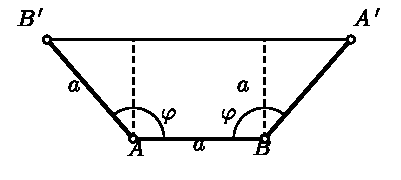
\includegraphics[width=5cm]{fig55.pdf}\\[0.3em]{\small 图 55}\end{minipage}\par\nopagebreak

现在绕通过 $A$ 的轴旋转角度 $\varphi=\dfrac{2\pi}{n}$（$n$ 是轴的重数）.于是 $B$ 点连同过它的轴移到 $B'$ 位置.类似地，绕 $B$ 的旋转把 $A$ 移到 $A'$.构造过程要求 $A'$ 和 $B'$ 属于同一个布拉维格子，因此可以通过平移相互重合.因此距离 $A'B'$ 也一定是晶格的一个周期.如果 $a$ 是在该方向的基本周期，那么距离 $A'B'$ 必然等于 $ap$，其中 $p$ 是整数.由图55看到，这给出方程式
\begin{equation*}
  a+2a\sin\left(\varphi-\frac{\pi}{2}\right)=a-2a\cos\varphi=ap,
\end{equation*}
即
\begin{equation*}
  \cos\varphi=\frac{1-p}{2}.
\end{equation*}
因为 $|\cos\varphi|\leqslant1$，所以 $p$ 可以等于$3,2,1,0$.这些值对应于在 $\varphi=\dfrac{2\pi}{n}$ 中取 $n=2,3,4,6$.因此，一个晶格只可能具有重数为2、3、4和6的旋转对称轴.

现在我们来讨论布拉维格子相对于旋转和反映的对称类型.这些对称类型称为晶系.每一个晶系是确定的一组对称轴和对称面，也就是一个点群.

很容易看出：布拉维格子的每一格点都是那里的对称中心.实际上，布拉维格子中的每一个原子有与之对应的另一原子，后者同前者及给定的格点共线，并且这两个原子与该格点等距.如果对称中心是布拉维格子除平移以外的唯一对称元素，那么有以下几种情况：

1. 三斜晶系.这种晶系在所有晶系中对称性最低，对应于点群 $C_i$.三斜布拉维格子的格点，位于棱长、棱角都是任意的全同平行六面体的顶点上；这样的平行六面体如图56所示.布拉维格子通常用专门的符号标记，三斜晶系记作 $\Gamma_t$.

\par\nopagebreak\noindent\begin{minipage}{\linewidth}\centering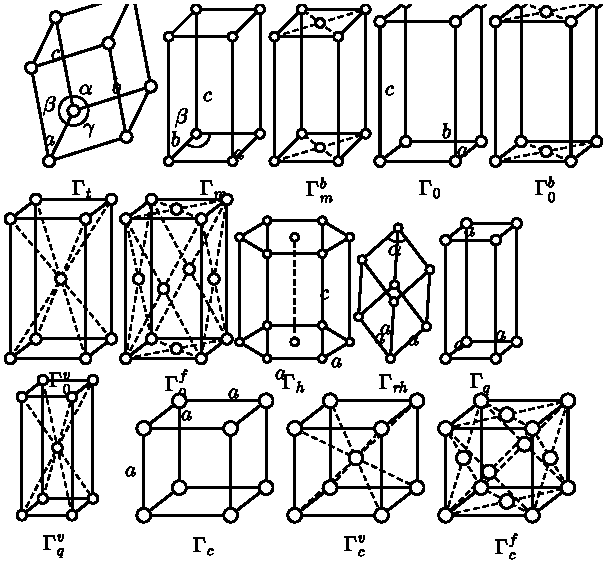
\includegraphics[width=10.5cm]{fig56.pdf}\\[0.3em]{\small 图 56}\end{minipage}\par\nopagebreak

2. 单斜晶系是对称性次低的晶系.它的对称元素是一个二重轴和一个与它垂直的对称面，也就是说这个晶系是点群 $C_{2h}$.这是底面任意的直平行六面体的对称.这种晶系的布拉维格子可以有两种构造方式.第一种情形称为简单单斜布拉维格子（$\Gamma_m$），格点位于以任意平行四边形作为面 $ac$ 而直边为 $b$ 的平行六面体的顶点上(图56).第二种情形是底心单斜格子（$\Gamma_m^b$），格点不仅位于平行六面体的顶点，而且还位于平行六面体的两个对立矩形面的中心.

3. 正交晶系对应于点群 $D_{2h}$.这是棱长任意的长方体的对称.属于正交晶系的有四种布拉维格子.在简单正交格子（$\Gamma_o$）中，格点位于长方体的顶点上.在底心格子（$\Gamma_o^b$）中，格点还位于每个长方体的一对对立面的中心.在体心格子（$\Gamma_o^v$）中，格点位于长方体的顶点和中心.最后，在面心格子（$\Gamma_o^f$）中，格点位于长方体的顶点及所有的面心.

4. 四方(或四角)晶系对应于点群 $D_{4h}$；这是四方柱体具有的对称.这种晶系的布拉维格子可以有两种方式；即简单的和体心的四方布拉维格子(记作 $\Gamma_q$ 和 $\Gamma_q^v$)，格点分别位于四方柱体的顶点，以及位于顶点和中心.

5. 三方(或三角)晶系对应于点群 $D_{3d}$；这是菱面体所具有的对称(菱面体是立方体沿着它的一根空间对角线拉长或压缩所形成的体).在这个晶系中唯一可能的布拉维格子（$\Gamma_{rh}$）中，格点位于菱面体的顶点.

6. 六方晶系对应于点群 $D_{6h}$；这是正六角柱体的对称.这种晶系的布拉维格子（$\Gamma_h$）只能以一种方式实现，即它的格点位于正六角柱体的顶点和六角形底面的中心.值得注意的，六方和三方布拉维格子之间有下述的区别.在这两种格子中，格点都位于与6重(或3重)轴的垂面中，构成等边三角网络.但是在六方格子中，在(沿着 $C_6$ 轴方向的)相继各平面中，格点一个在另一个的正上方(这些平面的示意图如图57所示).至于三方格子，则每一平面的格点都在前一平面的格点所构成三角形的中心之上(如图57中的小圈和小叉).

\par\nopagebreak\noindent\begin{minipage}{\linewidth}\centering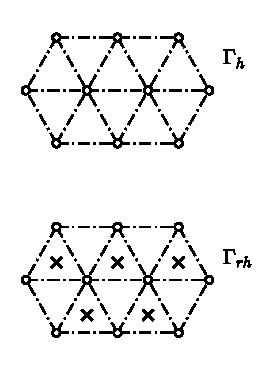
\includegraphics[width=7cm]{fig57.pdf}\\[0.3em]{\small 图 57}\end{minipage}\par\nopagebreak

7. 立方晶系对应于点群 $O_h$；这是立方体的对称.属于这种晶系的有三种布拉维格子：简立方（$\Gamma_c$）、体心立方（$\Gamma_c^v$）和面心立方（$\Gamma_c^f$）.

在三斜、单斜、正交、四方、立方这个晶系序列中，每一晶系都比它前面的所有晶系具有更高的对称.换句话说，后面晶系包含前面晶系出现的所有对称元素.在这种意义下，三方晶系所具备的对称高于单斜晶系，而同时低于立方和六方晶系，这后二者都包含三方晶系的对称元素，即这两种晶系最为对称.

值得注意的还有下述情况.乍看起来，除了上面所列举的14种布拉维格子以外，似乎还可能有其它类型，例如对于简单四方格子，如果在柱体的上、下正方底面中心加上格点，那么这个格子仍有原先的四角对称.但是很容易看出，这里并没有得到新的布拉维格子.实际上，如果图58所示的方式用虚线联结这个格子的格点，那么我们看到新格子仍为简单四方.很容易证实，所有其它类似情形也是如此.

\par\nopagebreak\noindent\begin{minipage}{\linewidth}\centering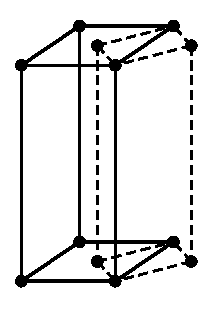
\includegraphics[width=4.5cm]{fig58.pdf}\\[0.3em]{\small 图 58}\end{minipage}\par\nopagebreak

图56中所表示的各布拉维格子的平行六面体，本身具有它们所属晶系的全部对称元素.但是必须注意：除了几种简单布拉维格子以外，这些平行六面体并不是原胞；构成这些平行六面体的周期不是基本周期.对于面心布拉维格子，可以选取从平行六面体的任一顶点到面心的矢量作为基本周期；而对于体心格子可取从平行六面体的顶点到体心的矢量；诸如此类.图59表示立方格子 $\Gamma_c^f$ 和 $\Gamma_c^v$ 的原胞；这两种原胞都是菱面体，它们本身并不具有立方晶系的全部对称元素.显然，面心布拉维六面体的体积 $v_f$ 是原胞体积的四倍：$v_f=4v$；体心平行六面体和底心六面体的体积等于原胞体积的二倍：$v_v=2v$，$v_b=2v$.

\par\nopagebreak\noindent\begin{minipage}{\linewidth}\centering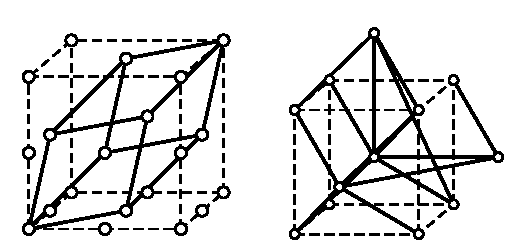
\includegraphics[width=8cm]{fig59.pdf}\\[0.3em]{\small 图 59}\end{minipage}\par\nopagebreak

完全确定一个三斜布拉维格子，必须指定六个量：平行六面体的棱长和棱角.对于单斜晶系，四个量就够了，因为有两个棱角总是直角；余可类推.类似的分析容易发现，确定各种晶系的布拉维格子所必需的量(平行六面体的棱长和棱角)的数目如下：
\begin{center}
\begin{tabular}{ll}
三斜系…6 & 三方系…2 \\
单斜系…4 & 六方系…2 \\
正交系…3 & 立方系…1 \\
四方系…2 &
\end{tabular}
\end{center}

\section{晶类}

对于所有可以称为是宏观的一系列现象来说，晶体的行为就像连续的均匀物质一样.晶体的诸多宏观性质仅仅与晶体中的方向有关.例如，光线通过晶体的特性只依赖于光线的方向；晶体的热膨胀在不同方向一般来讲是不同的；最后，晶体在各种外力影响下的弹性形变也依赖于方向.

另一方面，晶体的对称导致晶体中不同方向的等价性.晶体的所有各种宏观性质，沿这些方向完全一样.因此，可以说晶体的宏观性质取决于晶体中的方向对称性.例如，如果晶体具有对称中心，那么晶体中的任何方向都和它的相反方向等效.

晶格的平移对称不导致任何方向上的等价性，因为平移根本不改变方向.由于这个缘故，对于方向对称来说，螺旋轴和简单对称轴之间或是滑移面和简单对称面之间的差别无关紧要.

因此，晶体的方向对称，进而它的宏观性质的对称，由它的一组对称轴和对称面来决定，而且螺旋轴和滑移面这时应看成是简单的轴和面.这样的对称元素集称为晶类.

我们已经知道，一个实际晶体可以看成是一组互穿的等同布拉维格子.由于布拉维格子的套叠，实际晶体的对称一般不同于相应的布拉维格子的对称.

特别是，一个给定晶体的晶类对称元素集，一般不同于其晶系.显然，新格点加到布拉维格子上，只可能使得它的某些对称轴和对称面消失，而不会出现新元素.因此，与晶类所对应的晶系相比，即与该晶体布拉维格子的对称轴和对称面总数相比，晶类所包含的对称元素数目较少(或至多相等).

由以上分析可以提出寻求属于一个给定晶系的所有晶类的方法.为此，必须求出由该晶系的全部或某些对称元素所构成的全部点群.但是，这样得到的点群其对称元素有可能不只属于一个晶系.例如，前节中已经看到：所有的布拉维格子都具有对称中心.因此所有的晶系都包含点群 $C_i$.虽然如此，不同晶系的晶类划分，通常有唯一的物理方式.这就是，每个晶类所划归的晶系，在含有该晶类的所有晶系之中必须对称性最低.例如，晶类 $C_i$ 必须归入只含反演中心而无任何其它对称元素的三斜晶系.这种晶类分法，绝不会把一个具有某种布拉维格子的晶体，归入一个可用对称性较低晶系的布拉维格子生成的晶类中(只有一个例外，见下).

满足这个条件的必要性在物理上很明显.实际上，晶体中属于其布拉维格子的原子按照比晶体对称所要求的更高对称方式配置，这在物理上极不可能.何况这样的位形即使偶然出现，那么任何外来影响(如加热)哪怕很弱也足以把它破坏，因为这种位形同晶体对称没有必然联系.举例来说，如果一个晶体属于一个由四方晶系就足以生成的晶类，假如它具备立方的布拉维格子，那么即使不很大的影响，也能引起立方原胞的一条棱伸长或缩短，而使它变成正方形棱柱体.

从这个例子可以看出起着重要作用的一个事实：高对称晶系的布拉维格子，可以通过微不足道的形变而变成低对称晶系的格子.但是也存在一个找不到这种变换的例外：用任何的无限小形变都不能使六方布拉维格子变成低对称的三方晶系格子.由图57可以看出：要把六方格子变成三方格子，每隔一层的格点必须位移一个有限距离，即从三角形的顶点移到中心.这导致三方晶系的全部晶类既可以由六方的，也可以由三方的布拉维格子来生成\footnote{通常把具有六方布拉维格子而属于三方晶类的晶体归入三方晶系.}.

因此，要找出所有的晶类，必须从寻找对称程度最低的晶系即三斜晶系的点群开始，然后依次过渡到较高对称的晶系，而同时把已经归入较低对称晶系的点群(即晶类)去掉.结果发现总共只有32个晶类存在；这些晶类按照晶系分类列表如下：
\begin{center}
\begin{tabular}{c|l}
\hline
晶系 & \multicolumn{1}{c}{晶类} \\
\hline
三斜 & $C_1$，\ $C_i$ \\
单斜 & $C_s$，\ $C_2$，\ $C_{2h}$ \\
正交 & $C_{2v}$，\ $D_2$，\ $D_{2h}$ \\
四方 & $S_4$，\ $D_{2d}$，\ $C_4$，\ $C_{4h}$，\ $C_{4v}$，\ $D_4$，\ $D_{4h}$ \\
三方 & $C_3$，\ $S_6$，\ $C_{3v}$，\ $D_3$，\ $D_{3d}$ \\
六方 & $C_{3h}$，\ $D_{3h}$，\ $C_6$，\ $C_{6h}$，\ $C_{6v}$，\ $D_6$，\ $D_{6h}$ \\
立方 & $T$，\ $T_h$，\ $T_d$，\ $O$，\ $O_h$ \\
\hline
\end{tabular}
\end{center}

上述晶类的每一组中，最后一个是对称性最高的一个，包含该晶系的全部对称元素.如果晶类的对称同它所在晶系的对称等同，就称这种晶类为全面象晶类.如果晶类所具备的各种对称变换(旋转和反映，并包括全等变换在内)的数目比全面象晶类小一因子二或四，那么就分别称它们为半面象或四分面象晶类.例如，在立方晶系中，$O_h$ 是全面象晶类，$O$、$T_h$、$T_d$ 是半面象晶类，而 $T$ 是四分面象晶类.

\section{空间群}

在研究了布拉维格子的对称和晶体的方向对称以后，我们可以最终考虑晶格全部的真实对称.这种对称可以称为微观对称，以区别于在上节中所讨论的晶体宏观对称.微观对称将决定晶体的依赖于原子在晶格中如何配置的性质(如晶体X射线散射).

晶格的(实际的)对称元素集合称为它的空间群.晶格总是具有确定的平移对称，除此以外，它还可能具有对称轴，如简单轴和螺旋轴、旋转反映轴以及对称面如简单面和滑移面.至于晶格的平移对称，则它完全由布拉维格子决定，因为后者的定义本身表明，除了布拉维格子周期以外，晶格没有其它平移周期.因此，要确定晶体的空间群，只需找出布拉维格子，并列举出与旋转和反映有关的对称元素.当然，同时还必须指出这些对称面和对称轴彼此间的相对位置.其次，必须注意到，晶格的平移对称意味着：如果晶格具备一个对称轴或对称面，它就会有无穷多个，且彼此只差一个等于晶格周期的平移.最后，除了这些相隔晶格周期的对称轴(或面)以外，平移对称和对称轴(或面)的同时存在，导致许多新轴(或面)的出现，后者不能通过平移任何晶格周期而与前者重合.例如，对称面的存在不仅导致出现与之平行的彼此相隔晶格周期的对称面，而且还出现平分这些周期的对称面.实际上很容易证实，对某一平面反映继而在垂直于该平面的方向位移距离 $d$，相当于取与之相距 $d/2$ 的平行平面作直接反映.

所有可能的空间群可按晶类划分.具体地说，如果在空间群的简单轴和螺旋轴之间及简单面和滑移面之间不予区别，这时一个空间群与某个晶类有相同的对称轴和对称面的集合，那么这个空间群划归该晶类.总共可能有230个不同的空间群存在\footnote{其中包括区别只在于绕螺旋轴的旋转方向的11对空间群.}.它们首先由费多罗夫（Е.~С.~Федоров，1895）发现.空间群按晶类的划分如表1.

\begin{center}
表1\\[0.8em]
\small\setlength{\tabcolsep}{3.5pt}
\begin{tabular}{cccccccc}
\hline
晶类 & 空间群数目 & 晶类 & 空间群数目 & 晶类 & 空间群数目 & 晶类 & 空间群数目 \\
\hline
$C_1$ & 1 & $S_4$ & 2 & $S_6$ & 2 & $C_{6v}$ & 4 \\
$C_i$ & 1 & $C_4$ & 6 & $C_{3v}$ & 6 & $D_6$ & 6 \\
$C_s$ & 4 & $C_{4h}$ & 6 & $D_3$ & 7 & $D_{6h}$ & 4 \\
$C_2$ & 3 & $D_{2d}$ & 12 & $D_{3d}$ & 6 & $T$ & 5 \\
$C_{2h}$ & 6 & $C_{4v}$ & 12 & $C_{3h}$ & 1 & $T_h$ & 7 \\
$C_{2v}$ & 22 & $D_4$ & 10 & $C_6$ & 6 & $T_d$ & 6 \\
$D_2$ & 9 & $D_{4h}$ & 20 & $C_{6h}$ & 2 & $O$ & 8 \\
$D_{2h}$ & 28 & $C_3$ & 4 & $D_{3h}$ & 4 & $O_h$ & 10 \\
\hline
\end{tabular}
\end{center}

我们不准备在这里列出全部空间群的对称元素，那是非常繁琐的.这可以在专门的晶体学参考书中找到\footnote{例如，空间群的详尽描述可以在下列书中找到：Любарский Г. Я. Теория групп и ее применения в физике (Приложение IV). Физматгиз, 1958; International Tables for Crystallography, v. A. Space Group Symmetry. -Dordrecht-Boston: D. Reidel Publishing Company, 1983. 后者还对每个空间群列举出全部等效点.}.

不含有螺旋轴或滑移面的空间群，称为点式空间群，这样的群共有73个.其余的157个空间群含有上述对称元素.属于非点式空间群的晶格，显然在一个原胞内至少应该含有两个同样的原子：绕螺旋轴转动或在滑移面内反映都涉及不足一个基本周期的平移，所以这种变换不能使布拉维格子的格点彼此重合，因而晶格必须至少由两个填以相同原子的互穿布拉维格子构成.

\section{倒格子}

所有表征晶格性质的物理量，都具有与晶格本身同样的周期性.例如，由晶格中原子的电子所产生的电荷密度，原子在晶格中处于任何一点的概率等都是这样的量.设函数 $U(\boldsymbol{r})$ 其中之一.其周期性表明
\begin{equation}
  U(\boldsymbol{r}+n_1\boldsymbol{a}_1+n_2\boldsymbol{a}_2+n_3\boldsymbol{a}_3)=U(\boldsymbol{r}),
\end{equation}
式中 $n_1,n_2,n_3$ 为任意整数，$\boldsymbol{a}_1,\boldsymbol{a}_2,\boldsymbol{a}_3$ 为晶格基本周期.

我们把周期函数 $U(\boldsymbol{r})$ 展开为三重傅里叶级数，展开式可写成
\begin{equation}
  U=\sum_{\boldsymbol{b}}U_{\boldsymbol{b}}\mathrm{e}^{\mathrm{i}\boldsymbol{b}\cdot\boldsymbol{r}},
\end{equation}
式中求和遍及矢量 $\boldsymbol{b}$ 的一切可能值.表示为级数形式(133.2)的函数 $U$ 必须满足周期性条件(133.1)，$\boldsymbol{b}$ 的可能取值由这一要求决定.这意味着：如果 $\boldsymbol{r}$ 换成 $\boldsymbol{r}+\boldsymbol{a}$（$\boldsymbol{a}$ 为任意周期），所有的指数因子都必须保持不变.为此，标量积 $\boldsymbol{a}\cdot\boldsymbol{b}$ 必须永远是 $2\pi$ 的整数倍.因此，依次选择基本周期 $\boldsymbol{a}_1,\boldsymbol{a}_2,\boldsymbol{a}_3$ 作为 $\boldsymbol{a}$，必定有
\begin{equation*}
  \boldsymbol{a}_1\cdot\boldsymbol{b}=2\pi p_1,\quad
  \boldsymbol{a}_2\cdot\boldsymbol{b}=2\pi p_2,\quad
  \boldsymbol{a}_3\cdot\boldsymbol{b}=2\pi p_3,
\end{equation*}
式中 $p_1,p_2,p_3$ 是正负整数或零.这三个方程式的解的形式为
\begin{equation}
  \boldsymbol{b}=p_1\boldsymbol{b}_1+p_2\boldsymbol{b}_2+p_3\boldsymbol{b}_3,
\end{equation}
式中矢量 $\boldsymbol{b}_i$ 通过矢量 $\boldsymbol{a}_i$ 决定如下：
\begin{equation}
  \boldsymbol{b}_1=\frac{2\pi}{v}\boldsymbol{a}_2\times\boldsymbol{a}_3,\quad
  \boldsymbol{b}_2=\frac{2\pi}{v}\boldsymbol{a}_3\times\boldsymbol{a}_1,\quad
  \boldsymbol{b}_3=\frac{2\pi}{v}\boldsymbol{a}_1\times\boldsymbol{a}_2,\quad
  v=\boldsymbol{a}_1\cdot(\boldsymbol{a}_2\times\boldsymbol{a}_3).
\end{equation}

这样我们就确定了矢量 $\boldsymbol{b}$ 的所有可能值.式(133.2)中的求和遍及 $p_1,p_2,p_3$ 的一切整数值.

大家知道，乘积 $v=\boldsymbol{a}_1\cdot(\boldsymbol{a}_2\times\boldsymbol{a}_3)$ 在几何上表示由矢量 $\boldsymbol{a}_1,\boldsymbol{a}_2,\boldsymbol{a}_3$ 所构成的平行六面体的体积，亦即原胞的体积；而乘积 $\boldsymbol{a}_1\times\boldsymbol{a}_2$ 等代表这个原胞的三个面的面积.因此，矢量 $\boldsymbol{b}_i$ 具有长度倒数的量纲，大小等于由矢量 $\boldsymbol{a}_1,\boldsymbol{a}_2,\boldsymbol{a}_3$ 所构成平行六面体的高的倒数乘以 $2\pi$.

由(133.4)可以看出：$\boldsymbol{b}_i$ 和 $\boldsymbol{a}_i$ 满足关系式
\begin{equation}
  \boldsymbol{a}_i\cdot\boldsymbol{b}_k=
  \begin{cases}
    0, & \text{如果 } i\neq k,\\
    2\pi, & \text{如果 } i=k.
  \end{cases}
\end{equation}
这意味着矢量 $\boldsymbol{b}_1$ 垂直于 $\boldsymbol{a}_2$ 和 $\boldsymbol{a}_3$，$\boldsymbol{b}_2$ 和 $\boldsymbol{b}_3$ 也类似.

在确定了矢量 $\boldsymbol{b}_i$ 以后，可以用 $\boldsymbol{b}_1,\boldsymbol{b}_2,\boldsymbol{b}_3$ 作为基本周期来形式地构造一个格子.这样构成的格子称为倒格子；矢量 $\boldsymbol{b}_1,\boldsymbol{b}_2,\boldsymbol{b}_3$ 称为倒格基矢\footnote{在现代物理学文献中采用的定义(133.4)，与纯结晶学中采用的定义相差一个因子$2\pi$.}.

我们现在来计算倒格子原胞的体积.它等于
\begin{equation*}
  v'=\boldsymbol{b}_1\cdot(\boldsymbol{b}_2\times\boldsymbol{b}_3).
\end{equation*}
把(133.4)式代入上式，得
\begin{equation*}
\begin{aligned}
  v'&=\frac{(2\pi)^3}{v^3}\,(\boldsymbol{a}_2\times\boldsymbol{a}_3)
  \cdot\left[(\boldsymbol{a}_3\times\boldsymbol{a}_1)
  \times(\boldsymbol{a}_1\times\boldsymbol{a}_2)\right]={}\\
  &=\frac{(2\pi)^3}{v^3}\left[(\boldsymbol{a}_2\times\boldsymbol{a}_3)
  \cdot\boldsymbol{a}_1\right]\cdot\left[(\boldsymbol{a}_3\times\boldsymbol{a}_1)
  \cdot\boldsymbol{a}_2\right],
\end{aligned}
\end{equation*}
最后得
\begin{equation}
  v'=\frac{(2\pi)^3}{v}.
\end{equation}

显然，三斜布拉维格子的倒格子原胞也是一个任意的平行六面体.类似地，其它晶系的简单布拉维格子其倒格子也是同一晶系的简单格子；例如，简立方布拉维格子的倒格子也具有简立方原胞.通过直接构造也很容易证实：面心布拉维格子(正交、四方、立方)的倒格子是同一晶系的体心格子；这时布拉维倒格子的平行六面体的体积 $v'_v=8(2\pi)^3/v_f$，式中 $v_f$ 是布拉维正格子平行六面体的体积.相反地，面心倒格子与体心正格子相对应，并且又有 $v'_f=8(2\pi)^3/v_v$.最后，对于底心正格子，其倒格子也具有底心的原胞，并且 $v'_b=4(2\pi)^3/v_b$.

大家知道，形如下式的方程
\begin{equation*}
  \boldsymbol{b}\cdot\boldsymbol{r}=\text{常数}
\end{equation*}
(式中 $\boldsymbol{b}$ 为常矢量)，描述一个垂直于矢量 $\boldsymbol{b}$ 的平面，它与原点的距离为 $\dfrac{\text{常数}}{b}$.选择布拉维格子的任何一个格点作为原点，并设 $\boldsymbol{b}=p_1\boldsymbol{b}_1+p_2\boldsymbol{b}_2+p_3\boldsymbol{b}_3$ 是倒格子的某一矢量（$p_1,p_2,p_3$ 为整数）.把 $\boldsymbol{r}$ 也写成 $\boldsymbol{a}=n_1\boldsymbol{a}_1+n_2\boldsymbol{a}_2+n_3\boldsymbol{a}_3$ 的形式，可得如下平面方程式
\begin{equation}
  \frac{\boldsymbol{b}\cdot\boldsymbol{a}}{2\pi}
  =n_1p_1+n_2p_2+n_3p_3=m,
\end{equation}
式中 $m$ 为给定常数.如果这个方程式代表一个有无数个布拉维格点的平面(通常叫做晶面)，那么 $n_1,n_2,n_3$ 必须是一组整数.为此，显然常数 $m$ 也必须是整数.在给定的 $p_1,p_2,p_3$ 下，当常数 $m$ 取不同整数值时，方程式(133.7)确定出无限多个相互平行的晶面.

整数 $p_1,p_2,p_3$ 总是可以取成互质的，即除1以外没有公约数.假如有这样的公约数存在，那么可以用它去除方程式的两边，而仍旧得到同样形式的方程式.数字 $p_1,p_2,p_3$ 称为这一族晶面的米勒指数，表示为 $(p_1p_2p_3)$.

晶面(133.7)与沿基本周期 $\boldsymbol{a}_1,\boldsymbol{a}_2,\boldsymbol{a}_3$ 取的坐标轴相交于 $\dfrac{m\boldsymbol{a}_1}{p_1},\dfrac{m\boldsymbol{a}_2}{p_2},\dfrac{m\boldsymbol{a}_3}{p_3}$ 三点.晶面在坐标轴上的截距(各以 $a_1,a_2,a_3$ 为单位来量度)之比为 $\dfrac{1}{p_1}:\dfrac{1}{p_2}:\dfrac{1}{p_3}$，即截距反比于米勒指数.例如，与坐标面平行的晶面(即在坐标轴上的截距之比为 $\infty:\infty:1$)，三个面分别有米勒指数 $(100)$，$(010)$，$(001)$.与晶格基本平行六面体的对角面平行的晶面具有指数 $(111)$，余类推.

很容易确定同一族晶面中相邻两面的间距.晶面(133.7)到原点的距离是 $\dfrac{2\pi m}{b}$，$b$ 是该倒格矢的长度.下一个晶面到原点的距离是 $\dfrac{2\pi(m+1)}{b}$.因此这两个晶面的间距 $d$ 是
\begin{equation}
  d=\frac{2\pi}{b}.
\end{equation}

在结束有关晶格对称性问题讨论之际，必须指出，严格的周期型晶体并未穷尽固体的所有可能类型.还存在所谓的无公度晶相，其密度函数 $\rho(x,y,z)$ 不是坐标的周期函数而只是条件周期的.表征该相性质的函数 $U(\boldsymbol{r})$ 的傅里叶级数(133.2)，其所含的矢量 $\boldsymbol{b}$ 将是三个以上基本周期的(整系数的)线性组合.

一般说来，前面所建立的周期晶体对称性质，对于无公度相不再成立.特别是它们可能具有的对称轴阶次不止是在§130中指出的那些.

\section{空间群的不可约表示}

对称性理论的物理应用通常用到所谓群表示这种数学工具.在本节我们将论述有关空间群的分类和构建其不可约表示的方法\footnote{这里假设读者熟悉类似于第三卷第12章中的有关群论知识.}.

我们先用比较数学化的术语重新概括在前几节表述的关于空间群结构的知识.

每个空间群都含有一个平移子群，它包含可使晶格与其自身重合的所有无限多个可能平移；这个子群也就是所谓晶体布拉维格子的数学表述.完全的空间群由这个子群再加上 $n$ 个旋转和反映的对称元素得到，$n$ 是相应晶类的对称变换数；这 $n$ 个元素将称为旋转元素.空间群的任何一个元素可以表示成一个平移元素与一个旋转元素的乘积\footnote{必须指出，平移子群是阿贝尔群(它的全部元素可对易)，而且是整个空间群的正规子群：与平移共轭的所有群元也是平移(两个元素$A$和$B$称为是共轭的，如果$A=C^{-1}BC$，而$C$也是群元).}.

如果一个空间群不包含螺旋轴和滑移面(点式空间群)，则旋转元素只能选晶类的 $n$ 个旋转和反映对称变换.但是，在非点式空间群中旋转元素是旋转和反映同时伴有某个基本周期的特定分数倍的平移.

为了便于清楚地表征空间群的元素，可用符号 $(P|\boldsymbol{t})$ 表示它们，这里 $P$ 是任何旋转或反映，而 $\boldsymbol{t}$ 是同时平移的矢量；当作用到任何一点的径矢 $\boldsymbol{r}$ 上时：$(P|\boldsymbol{t})\boldsymbol{r}=P\boldsymbol{r}+\boldsymbol{t}$.两个元素的相乘按照明显的法则：
\begin{equation}
  (P'|\boldsymbol{t}')(P|\boldsymbol{t})=(P'P|P'\boldsymbol{t}+\boldsymbol{t}').
\end{equation}
元素 $(P|\boldsymbol{t})$ 的逆元是
\begin{equation}
  (P|\boldsymbol{t})^{-1}=(P^{-1}|-P^{-1}\boldsymbol{t});
\end{equation}
它与 $(P|\boldsymbol{t})$ 相乘时，给出群的单位元 $(E|0)$（式中 $E$ 记恒等旋转变换）.

特别是，纯平移表示为 $(E|\boldsymbol{a})$，式中 $\boldsymbol{a}$ 是晶格任何周期.点式空间群的旋转元素，依上述方式选取则形为 $(P|0)$.在非点式空间群中，旋转元素的形式为 $(P|\boldsymbol{\tau})$，式中 $\boldsymbol{\tau}$ 是沿螺旋轴或滑移面发生的分数倍晶格周期的平移.在第一种情形下，旋转变换 $(P|0)$ 的集合本身形成空间群的子群.而在第二种情形下，元素 $(P|\boldsymbol{\tau})$ 本身并不形成子群，因为重复应用它们导致的不是恒等变换，而是某个晶格基本周期的平移.但是，像这样的转动与反映 $P$(也就是说对简单轴和螺旋轴或是简单面和滑移面不加区别)总是组成一个群即决定晶类的点对称群；就此而言，这个点群可称为晶格的方向群\footnote{在各种情况下，空间群与方向群之间的关系从群论的观点看来可以用如下方式表述.把空间群的所有元素按$n$个陪集分解，其中每一个包含一个旋转元素与所有可能平移的乘积的无穷集合，即给定$P$和$\boldsymbol{\tau}$下的形为$(P|\boldsymbol{\tau}+\boldsymbol{a})$的全部元素.如果现在把每个陪集整体上看成新群的元素，则得到原空间群的所谓商群.这个商群与方向群同构.}.

下面我们来构造空间群的不可约表示\footnote{下述推导由塞茨(F. Seitz, 1936)给出.}.

所有这种表示都可以用如下形式的函数集实现
\begin{equation}
  \varphi_{\boldsymbol{k}\alpha}=u_{\boldsymbol{k}\alpha}
  \mathrm{e}^{\mathrm{i}\boldsymbol{k}\cdot\boldsymbol{r}},
\end{equation}
式中 $\boldsymbol{k}$ 是常波矢，$u_{\boldsymbol{k}\alpha}$ 是相对于平移不变的函数；指标 $\alpha=1,2,\cdots$ 把具有相同 $\boldsymbol{k}$ 的函数编号.作为平移 $\boldsymbol{r}\to\boldsymbol{r}+\boldsymbol{a}$（式中 $\boldsymbol{a}$ 是晶格的任何一个周期）的结果，函数(134.3)被乘以常数 $\mathrm{e}^{\mathrm{i}\boldsymbol{k}\cdot\boldsymbol{a}}$.换而言之，在函数(134.3)实现的表示中，平移矩阵是对角的.显然，相差任何一个倒格子周期 $\boldsymbol{b}$ 的两个矢量 $\boldsymbol{k}$ 将导致函数 $\varphi_{\boldsymbol{k}\alpha}$ 在平移变换下具有同样的变换规律：因为 $\boldsymbol{a}\cdot\boldsymbol{b}$ 是 $2\pi$ 的整数倍，所以 $\exp(\mathrm{i}\boldsymbol{a}\cdot\boldsymbol{b})=1$.这样的矢量将称为是等效的.如果设想矢量 $\boldsymbol{k}$ 是从倒格子原胞的顶点引到其各点，那么所有不等效的矢量只限于一个原胞内.

在旋转对称元素 $(P|\boldsymbol{\tau})$ 的作用下，函数 $\varphi_{\boldsymbol{k}\alpha}$ 变换成矢量 $\boldsymbol{k}'$ 的不同 $\alpha$ 值函数 $\varphi_{\boldsymbol{k}'\alpha}$ 的线性组合，这里的 $\boldsymbol{k}'$ 由矢量 $\boldsymbol{k}$ 在倒格子中作给定的旋转或反映得到：$\boldsymbol{k}'=P\boldsymbol{k}$\footnote{对于矢量$\boldsymbol{k}$在倒格子中的变换，不言而喻，所有的对称轴和对称面都应当看成是简单的，即只应当考虑方向群.}.在群的全部 $n$ 个旋转元素的作用下可以相互转换的所有(非等效)矢量 $\boldsymbol{k}$ 的集合，称为波矢量 $\boldsymbol{k}$ 的波矢星.在任意 $\boldsymbol{k}$ 的一般情形下，波矢星含有 $n$ 个矢量(射线).含有波矢星的各射线的函数全应在不可约表示的基矢函数 $\varphi_{\boldsymbol{k}\alpha}$ 之内：因为含有不等效 $\boldsymbol{k}$ 的函数在平移下乘了不同的因子，所以无论怎样选择它们的线性组合作为可相互变换函数，函数的数目都不会减少.

对于某些k值，其波矢星的射线数可以少于 $n$，因为可能有些旋转对称元素并不改变k或者把它转变成等效矢量.例如，如果矢量k沿对称轴，则在绕该轴旋转时矢量不变；从原胞的顶点到它的中心的矢量 $\boldsymbol{k}$（$\boldsymbol{k}=\boldsymbol{b}_i/2$，式中 $\boldsymbol{b}_i$ 是倒格子的基本周期之一），在反演时变成与它等效的矢量 $-\boldsymbol{k}=-\boldsymbol{b}_i/2=\boldsymbol{k}-\boldsymbol{b}_i$.

包含在给定空间群内而且不改变矢量k(或者把它变为等效矢量)的那些对称旋转元素(全当作简单旋转或者反映 $P$)的集合，称为矢量k的“纯对称群”或就叫波矢群；它也是通常的点对称群之一.

我们首先考虑点式空间群的最简单情形.这种群的不可约表示的基函数可以写成乘积的形式：
\begin{equation}
  \varphi_{\boldsymbol{k}\alpha}=u_\alpha\psi_{\boldsymbol{k}},
\end{equation}
式中函数 $u_\alpha$ 相对于平动变换不变，而 $\psi_{\boldsymbol{k}}$ 是表达式 $\mathrm{e}^{\mathrm{i}\boldsymbol{k}\cdot\boldsymbol{r}}$(取等效的k)的线性组合，后者在矢量k的纯对称群的所有变换下不变；(134.4)中的矢量k取自己波矢星中所有值.在平移变换下函数 $u_\alpha$ 不变，而函数 $\psi_{\boldsymbol{k}}$(还有 $\varphi_{\boldsymbol{k}\alpha}$)被乘以 $\exp(\mathrm{i}\boldsymbol{k}\cdot\boldsymbol{a})$.在属于k群的旋转和反映之下，函数 $\psi_{\boldsymbol{k}}$ 不变，而函数 $u_\alpha$ 相互转换.换句话说，函数 $u_\alpha$ 实现了点群的一个不可约表示(由于这个缘故，可称之为“小表示”).最后，不在k群内的旋转元素使具有不等效k的函数(134.4)的集合彼此变换.用这种方式构造的空间群表示的维数等于k的波矢星中的射线数乘以小表示的维数.

因此，求点式空间群的所有不可约表示的问题完全归结为把矢量k按其纯对称性进行分类以及已解决的寻求有限点群不可约表示问题.

现在我们转向具有螺旋轴或滑移面的空间群.如果波矢k在它的群中所有变换下总不改变(即不转变为等效矢量)\footnote{具体说，这总包括矢量$\boldsymbol{k}=0$以及恒等变换为其波矢群单位元素的位置一般的矢量.}，这些对称元素的存在仍然是非本质的.这时相应的不可约表示仍然由形为(134.4)的函数实现，其中 $u_\alpha$ 形成矢量k的点群表示的基.与点式空间群情况的唯一区别就在于：在旋转变换下，(134.4)中的函数 $\psi_{\boldsymbol{k}}=\exp(\mathrm{i}\boldsymbol{k}\cdot\boldsymbol{r})$ 不再保持不变，而被乘以 $\exp(\mathrm{i}\boldsymbol{k}\cdot\boldsymbol{\tau})$.

但是，如果有多个等效的矢量k可在纯对称群的变换下相互转换，形为(134.4)的函数不再适用.在同时伴有平移 $\boldsymbol{\tau}$ 的旋转变换下，k值等效却不相同的函数 $\exp(\mathrm{i}\boldsymbol{k}\cdot\boldsymbol{r})$ 被乘上不同的因子（因为 $\boldsymbol{b}\cdot\boldsymbol{\tau}/2\pi$ 不是整数），所以它们的线性组合 $\psi_{\boldsymbol{k}}$ 不再变换到自身.

这时已不可能将旋转元素和平移分开考虑.但是，可以只考虑平移的无穷集合中的有限个，而且仅须对从倒格子原胞的顶点引到原胞内部某些选定点的矢量考虑；这些点的坐标(全部三个或其中几个)可用基本周期 $\boldsymbol{b}_1,\boldsymbol{b}_2,\boldsymbol{b}_3$ 的简单有理分数部分\footnote{实际上这些分数常常只取$\frac{1}{2}$,$\frac{1}{3}$,$\frac{2}{3}$(后两种值只出现在斜方六面体晶系与六方晶系的群中).}表示.由旋转元素(连同与其相伴的分数基本周期的平移 $\boldsymbol{\tau}$)以及 $\boldsymbol{k}\cdot\boldsymbol{a}/2\pi$ 为有理分数(小于1)的平移所组成的群，称为扩展波矢群；其余平移依旧可以认为是恒等变换.可对这样构成的有限群给出不可约表示(“小表示”)的函数 $\varphi$，连同 $\boldsymbol{k}$ 的波矢星其它射线对应的类似函数 $\varphi_{\boldsymbol{k}\alpha}$，可实现空间群的不可约表示.这里指出，这些群小表示的维数可达到6(晶类 $O_h$ 的群)\footnote{如果把扩展波矢群的表示看成非扩展群(点群之一)的表示，则群元$G$的表示阵$\hat{G}$之间的关系式会与群元素本身之间的关系式不同：假如$G_1G_2=G_3$，则相应表示阵之间的关系式一般并非为同样的等式$\hat{G}_1\hat{G}_2=\hat{G}_3$(如同通常的表示)，而是形为$\hat{G}_1\hat{G}_2=\omega_{12}\hat{G}_3$，式中$\omega_{12}$是某个相因子，仅仅模为1：$|\omega_{12}|=1$.这些表示称为射影表示.可以对于每个点群一次性地列出所有实质上不同的射影表示，然后将之用作小表示去构造空间群的不可约表示.
射影表示理论的论述和结晶学点群的射影表示图表可在下列书中找到：Бир Г Л, Пикус Г Е. Симметрия и деформационные эффекты в полупроводниках. – М.: Наука, 1972.
另有空间群不可约表示的完全表，见：Ковалев О В. Неприводимые и индуцированные представления и копредставления федоровских групп. – М.: Наука, 1986; Bradley C J, Cracknell A P. The mathematical theory of symmetry in solids. Oxford: Clarendon Press, 1972.}.

我们以具体的例子说明这种方法.

我们考虑空间群 $D_{2h}^2$，它属于简单斜方布拉维格子并包含下列的旋转元素\footnote{空间群通常用晶类符号标记并附加上标记群在该类中的编号.}：
\begin{equation*}
  (E|0),\ (C_2^x|0),\ (C_2^y|0),\ (C_2^z|0),\ (I|\boldsymbol{\tau}),\
  (\sigma_x|\boldsymbol{\tau}),\ (\sigma_y|\boldsymbol{\tau}),\
  (\sigma_z|\boldsymbol{\tau}),
\end{equation*}
式中 $x,y,z$ 轴沿晶格的三个基本周期取，而 $\boldsymbol{\tau}=(\boldsymbol{a}_1+\boldsymbol{a}_2+\boldsymbol{a}_3)/2$(对称轴 $C_2$ 是简单的，而与之垂直的平面 $\sigma$ 是滑移面).

例如，我们选取矢量
\begin{equation}
  \boldsymbol{k}=(1/2,0,0),
\end{equation}
式中括号内的数字给出矢量沿倒格子轴的分量并以其原胞的棱长 $(b_i=2\pi/a_i)$ 为量度单位.这个波矢量的纯对称含有点群 $D_{2h}$ 的全部对称轴与对称面，因此这个矢量本身组成波矢星.附加上满足 $\boldsymbol{k}\cdot\boldsymbol{a}/2\pi=1/2$ 的平移 $(E|\boldsymbol{a}_1)$，得到扩展群.结果，我们得到由16个元素分成10类组成的群，如表2的最上一行所示.二元素如 $(C_2^y|0)$ 和 $(C_2^y|\boldsymbol{a}_1)$ 的共轭性(即同属一类)，可证实如下.我们有

\begin{center}
表2\\[0.8em]
\small\setlength{\tabcolsep}{2.5pt}
\begin{tabular}{lcccccccccc}
\hline
 & $(E|0)$ & $(E|\boldsymbol{a}_1)$ & $(C_2^x|0)$ & $(C_2^x|\boldsymbol{a}_1)$
 & \shortstack{$(C_2^y|0)$\\$(C_2^y|\boldsymbol{a}_1)$}
 & \shortstack{$(C_2^z|0)$\\$(C_2^z|\boldsymbol{a}_1)$}
 & \shortstack{$(I|\boldsymbol{\tau})$\\$(I|\boldsymbol{\tau}+\boldsymbol{a}_1)$}
 & \shortstack{$(\sigma_x|\boldsymbol{\tau})$\\$(\sigma_x|\boldsymbol{\tau}+\boldsymbol{a}_1)$}
 & \shortstack{$(\sigma_y|\boldsymbol{\tau})$\\$(\sigma_y|\boldsymbol{\tau}+\boldsymbol{a}_1)$}
 & \shortstack{$(\sigma_z|\boldsymbol{\tau})$\\$(\sigma_z|\boldsymbol{\tau}+\boldsymbol{a}_1)$} \\
\hline
$\Gamma_1$ & 2 & $-2$ & 2 & $-2$ & 0 & 0 & 0 & 0 & 0 & 0 \\
$\Gamma_2$ & 2 & $-2$ & $-2$ & 2 & 0 & 0 & 0 & 0 & 0 & 0 \\
\hline
\end{tabular}
\end{center}

\begin{equation*}
\begin{aligned}
  (I|\boldsymbol{\tau})^{-1}(C_2^y|0)(I|\boldsymbol{\tau})
  &=(I|-\boldsymbol{\tau})(C_2^y|0)(I|\boldsymbol{\tau})={}\\
  &=(I|-\boldsymbol{\tau})(C_2^y I|C_2^y\boldsymbol{\tau})
  =(C_2^y|-\boldsymbol{\tau}+C_2^y\boldsymbol{\tau}).
\end{aligned}
\end{equation*}
但是
\begin{equation*}
  C_2^y\boldsymbol{\tau}=\frac{1}{2}(-\boldsymbol{a}_1+\boldsymbol{a}_2-\boldsymbol{a}_3),\qquad
  C_2^y\boldsymbol{\tau}-\boldsymbol{\tau}=-\boldsymbol{a}_1-\boldsymbol{a}_3
  =\boldsymbol{a}_1-(2\boldsymbol{a}_1+\boldsymbol{a}_3),
\end{equation*}
而因为依 $\boldsymbol{a}_3$ 和 $2\boldsymbol{a}_1$ 的平移应该看成恒等变换，所以
\begin{equation*}
  (I|\boldsymbol{\tau})^{-1}(C_2^y|0)(I|\boldsymbol{\tau})=(C_2^y|\boldsymbol{a}_1).
\end{equation*}

根据群的元素数与类数，我们求出它有8个一维的和两个二维的不可约表示（$8\cdot1^2+2\cdot2^2=16$）.所有的一维表示可从点群 $D_{2h}$ 的表示得出，并且赋予平移 $(E|\boldsymbol{a}_1)$ 特征标1.然而，这里生成的这些表示是“虚假的”，应舍弃.它们并不对应于这里的问题：它们的基函数相对于所有的平移不变，而给定k的函数 $\mathrm{e}^{\mathrm{i}\boldsymbol{k}\cdot\boldsymbol{r}}$ 在平移 $(E|\boldsymbol{a}_1)$ 下必定改变.这样，只留下两个不可约表示，它们的特征标已在表2中列出.这些表示的基函数可选
\begin{equation*}
\begin{aligned}
  \Gamma_1&:\ \cos\pi x,\quad \sin\pi x,\\
  \Gamma_2&:\ \cos\pi x\,\sin2\pi y,\quad \sin\pi x\,\sin2\pi y
\end{aligned}
\end{equation*}
(坐标 $x,y,z$ 分别用相应的基本周期 $\boldsymbol{a}_1,\boldsymbol{a}_2,\boldsymbol{a}_3$ 的长度来量度).

我们再考虑与以下两个矢量的波矢星对应的表示：
\begin{equation}
  \boldsymbol{k}=(1/2,0,\varkappa),\quad (1/2,0,-\varkappa)
\end{equation}
它们具有纯对称 $C_{2v}$（$C_2$ 的轴沿z轴）；式中 $\varkappa$ 是0和1之间的任意数（但 $\dfrac{1}{2}$ 除外）.$\boldsymbol{k}$ 的扩展群包含分成5类的8个元素(表3).(这个群的表示基函数与z的依赖关系归结为共同的因子 $\exp(2\pi\mathrm{i}\varkappa z)$ 或 $\exp(-2\pi\mathrm{i}\varkappa z)$，它们在群的所有变换下不变；因此，不必用沿z轴的平移来扩展群.)该群存在4个一维的和一个二维的不可约表示.

\begin{center}
表3\\[0.8em]
\small\setlength{\tabcolsep}{3pt}
\begin{tabular}{ccccc}
\hline
$(E|0)$ & $(E|\boldsymbol{a}_1)$
& \shortstack{$(C_2^x|0)$\\$(C_2^x|\boldsymbol{a}_1)$}
& \shortstack{$(\sigma_x|\boldsymbol{\tau})$\\$(\sigma_x|\boldsymbol{\tau}+\boldsymbol{a}_1)$}
& \shortstack{$(\sigma_y|\boldsymbol{\tau})$\\$(\sigma_y|\boldsymbol{\tau}+\boldsymbol{a}_1)$} \\
\hline
2 & $-2$ & 0 & 0 & 0 \\
\hline
\end{tabular}
\end{center}

根据与上述情形同样的理由，应该丢弃一维表示，因此只剩下一个表示，其特征标在表3中给出.它的基函数可以选为如下形式
\begin{equation*}
  \mathrm{e}^{\pm2\pi\mathrm{i}\varkappa z}\cos\pi x,\qquad
  \mathrm{e}^{\pm2\pi\mathrm{i}\varkappa z}\sin\pi x.
\end{equation*}
指数中的正负号分别与(134.6)中的第一和第二矢量对应；整个空间群完整的不可约表示为四维，并且用这组全部四个函数实现.

\section{时间反演对称性}

在对称群理论的物理学应用中，通常还对群表示附加以下要求：表示的基函数必须是实的(更确切地说，可化为实的形式).此要求是时间反演对称的结果.在量子力学中，由于这种对称性，互为复共轭的波函数必须对应于量子系统的同一个能级，因此必须出现在同一个物理不可约表示的基函数中(参看第三卷§96).在经典理论中这种对称性用运动方程对于替换 $\boldsymbol{t}\to-\boldsymbol{t}$ 的不变性来表达(方程式含有对时间的偶数阶——2阶导数).正是因这一点，在寻求解为复数形式 $(\propto\mathrm{e}^{-\mathrm{i}\omega t})$ 的(69.6)时，原子在晶格中位移 $u_s$ 的方程仍然是实的；于是这些表达式的振幅可以取为实的\footnote{但是在有磁场时或具有磁结构的晶体中，情况已经不再是这样.}.

当然实的基函数在所有对称元素作用下仍旧是实的；换而言之，群表示的所有矩阵也都是实的.如果某个不可约表示不满足这个要求，则它必须同其复共轭表示联合成一个维数加倍的物理不可约表示.让我们从这个观点出发，考虑在空间群表示中可以出现的情况（C.~Herring，1937）.

在这一方面，最简单的情况是当波矢k与−k的波矢星彼此不一致的时候.这时从二波矢星中每一个建立起来的不可约表示显然都是复的.例如，对于k波矢星而言，表示的基函数在平移 $(E|\boldsymbol{a})$ 下应乘以因子 $\mathrm{e}^{\mathrm{i}\boldsymbol{k}\cdot\boldsymbol{a}}$，而这些因子之间不相互复共轭；因此很明显，无论如何选择这些函数的线性组合，都不能把变换阵化为实形式.另一方面，取这些函数的复共轭可得到复共轭的属于矢量−k波矢星的表示.这两种表示联合可得实表示.因此，为得出物理不可约表示，对每个k必须把矢量−k也一起包括在波矢星中.换句话说，为了得到需要的整个波矢星，必须将方向群的所有元素并加上对称中心作用于某个原始的k.

假如波矢星已经从一开始就包含全部需要的k值，但是这还是不能保证在其上构建的不可约表示是实的.我们用简单的例子来说明.

考虑属于晶类 $S_4$ 并具有简单四方布拉维晶格的点式空间群 $S_4^1$.在该群中取出与以下两个矢量的波矢星对应的表示：
\begin{equation}
  \boldsymbol{k}=(0,0,\varkappa),\quad (0,0,-\varkappa),
\end{equation}
式中z轴沿对称轴 $S_4$，而 $\varkappa$ 是0和1之间的任意数（但 $\dfrac{1}{2}$ 除外）.这两个矢量的纯对称群是 $C_2$，这个点群有两个一维表示，它们的特征标分别为
\begin{center}
\begin{tabular}{lcc}
\hline
 & $E$ & $C_2$ \\
\hline
$A$ & 1 & 1 \\
$B$ & 1 & $-1$ \\
\hline
\end{tabular}
\end{center}
取其中第一个作为小表示，我们得到整个空间群的一个二维表示，表示基可以取为复共轭形式的函数 $\exp(\pm2\pi\mathrm{i}\varkappa z)$；因此这个表示是实的.与小表示B对应的整个群的二维表示由以下基函数实现：
\begin{equation*}
  \exp(2\pi\mathrm{i}\varkappa z)\cos2\pi x,\qquad
  \exp(-2\pi\mathrm{i}\varkappa z)\sin2\pi x.
\end{equation*}
在这个表示中群的旋转元素的特征标为
\begin{equation*}
\begin{array}{ccccc}
  (E|0) & (S_4|0) & (C_2|0) & (S_4^3|0) & \\
  2 & 0 & -2 & 0 & ,
\end{array}
\end{equation*}
而平移的特征标为
\begin{equation*}
\begin{array}{cccc}
  (E|\boldsymbol{a}_1) & (E|\boldsymbol{a}_2) & (E|\boldsymbol{a}_3) & \\
  2 & 2 & 2\cos2\pi\varkappa & .
\end{array}
\end{equation*}
所有这些特征标都是实的，然而表示却是复的：它的基函数不可能转变成实的形式.这些函数加上其复共轭，亦即将等价的(具有同样特征标)两个复共轭表示\footnote{值得提醒，在点群中这种情况不会发生：对于这些群所有具有实特征标的不可约表示都是实的.}联合起来，可得到物理上的不可约表示.

在已考虑的例子中，对于k空间中填满直线(对称轴)的波矢值，时间反演对称导致物理不可约表示的维数加倍.这样的加倍情况也发生于k值填满k空间的整个平面时，这里说的平面垂直于二重螺旋轴.

我们再考虑一个非点式空间群 $C_2^2$ 的例子，这个群属于晶类 $C_2$ 而且具有简单单斜布拉维晶格.其中二重轴(取作z轴)是螺旋轴，带有半个周期的平移：$(C_2|\boldsymbol{a}_3/2)$.对于这个群考虑以下两个波矢的波矢星：
\begin{equation}
  \boldsymbol{k}=(\varkappa,\Lambda,1/2),\quad (-\varkappa,-\Lambda,1/2),
\end{equation}
式中 $\varkappa$ 和 $\Lambda$ 是0与 $\dfrac{1}{2}$ 之间的任意数(x轴和y轴斜交，在垂直于对称轴的平面中)；波矢星包含k和−k在内，因为矢量 $(\varkappa,\Lambda,1/2)$ 和 $(-\varkappa,-\Lambda,1/2)$ 是等效的.该波矢星对应于两个等效的(具有相同实特征标的)二维不可约群表示，分别由以下的基函数及其复共轭实现：
\begin{equation*}
  \mathrm{e}^{\pm2\pi\mathrm{i}(\varkappa x+\Lambda y)}\mathrm{e}^{\mathrm{i}\pi z}.
\end{equation*}
物理不可约表示可由联合这两个复共轭表示得到.它的四个基函数分成两对，各对应于波矢星中两个波矢之一：
\begin{equation*}
  \mathrm{e}^{2\pi\mathrm{i}(\varkappa x+\Lambda y)}\mathrm{e}^{\pm\mathrm{i}\pi z},\qquad
  \mathrm{e}^{-2\pi\mathrm{i}(\varkappa x+\Lambda y)}\mathrm{e}^{\pm\mathrm{i}\pi z}.
\end{equation*}

如果不可约表示与它的基函数一起已经找到，关于它是实是复的问题，答案变得很明显.然而在更复杂的情况下(也为了研究某些更一般的问题)，如果有一个判据可供从小表示特征标直接回答这个问题，是十分有用的.从以下群表示论的普遍定理出发，能够得出这样的判据\footnote{它的证明可参阅§132最后一个和§134倒数第二个脚注所列书籍.}.

对于群的每个不可约表示，以下和式可以取三个值中之一：
\begin{equation}
  \frac{1}{g}\sum_G\chi(G^2)=
  \begin{cases}
    +1 & \text{(a)},\\
    0 & \text{(b)},\\
    -1 & \text{(c)}
  \end{cases}
\end{equation}
(求和遍及所有群元，g是群的阶).根据这些数值：(a)表示为实的；(b)表示为复的，并且与其复共轭的表示不等价(有复共轭特征标)；(c)表示为复的，并且与其复共轭的表示等价(有同样的实特征标).

略去细节，我们将概述如何改写这个判据以便用于空间群.根据上节所述的构建空间群不可约表示的方法，特征标可以表示为
\begin{equation}
  \chi[(P|\boldsymbol{\tau}+\boldsymbol{a})]
  =\sum_i\chi_{\boldsymbol{k}_i}[(P|\boldsymbol{\tau})]
  \exp(\mathrm{i}\boldsymbol{k}_i\cdot\boldsymbol{a}),
\end{equation}
式中 $\chi_{\boldsymbol{k}}[(P|\boldsymbol{\tau})]$ 是群旋转元素的小表示特征标，求和遍及波矢星的以 $P$ 为其对称群元素之一的那些射线 $\boldsymbol{k}_1,\boldsymbol{k}_2,\cdots$.把这个公式用于元素
\begin{equation*}
  (P|\boldsymbol{\tau}+\boldsymbol{a})^2
  =(P^2|\boldsymbol{\tau}+P\boldsymbol{\tau}+\boldsymbol{a}+P\boldsymbol{a})
  =(P|\boldsymbol{\tau})^2(E|\boldsymbol{a}+P\boldsymbol{a}),
\end{equation*}
我们有
\begin{equation*}
  \chi[(P|\boldsymbol{\tau}+\boldsymbol{a})^2]
  =\sum_i\chi_{\boldsymbol{k}_i}[(P|\boldsymbol{\tau})^2]
  \exp[\mathrm{i}\boldsymbol{a}\cdot(\boldsymbol{k}_i+P^{-1}\boldsymbol{k}_i)]
\end{equation*}
(在指数中已作代换 $\boldsymbol{k}_i\cdot P\boldsymbol{a}
=\boldsymbol{a}\cdot P^{-1}\boldsymbol{k}_i$).这些特征标应该对所有的平移和所有的旋转元素 $(P|\boldsymbol{\tau})$ 求和.和式
\begin{equation*}
  \sum_{\boldsymbol{a}}\exp[\mathrm{i}\boldsymbol{a}\cdot(\boldsymbol{k}_i+P^{-1}\boldsymbol{k}_i)]
\end{equation*}
仅在 $\boldsymbol{k}_i+P^{-1}\boldsymbol{k}_i=0,\boldsymbol{b}$ 时不为零.最后注意到，由于在(最后应计算的)对i求和中波矢星所有射线等价，所有各项相同.

结果我们得到以下最终的Herring判据：
\begin{equation}
  \frac{1}{n_{\boldsymbol{k}}}\sum\chi_{\boldsymbol{k}}[(P|\boldsymbol{\tau})^2]=
  \begin{cases}
    +1 & \text{(a)},\\
    0 & \text{(b)},\\
    -1 & \text{(c)},
  \end{cases}
\end{equation}
式中 $\chi_{\boldsymbol{k}}$ 是小表示的特征标，而取求和所遍及可将k变换成−k的等效矢量即 $P\boldsymbol{k}=-\boldsymbol{k}+\boldsymbol{b}$ 的空间群旋转元素\footnote{这时$(P|\boldsymbol{\tau})^2$不改变矢量$\boldsymbol{k}$(或者把它转变成等效的)，即显然包含在矢量$\boldsymbol{k}$的纯对称群内.}；$n_{\boldsymbol{k}}$ 是波矢纯对称群中旋转元素的数目.

特别是，假如空间群完全不含具有所指定性质的旋转元素，则和式(135.5)中一项也没有，因此出现情况(b)，这与前面讨论过的k与−k有不同波矢星的情形一致.

在前面所考虑的群 $S_4^1$ 的例子中，元素 $(S_4|0)$ 和 $(S_4^3|0)$ 具有所要求的性质；它们的平方是元素 $(C_2|0)$.所以和式(135.5)为
\begin{equation*}
  \frac{1}{2}\left\{\chi_{\boldsymbol{k}}[(S_4|0)^2]
  +\chi_{\boldsymbol{k}}[(S_4^3|0)^2]\right\}
  =\chi_{\boldsymbol{k}}[(C_2|0)];
\end{equation*}
对于小表示A它等于+1，对于小表示B等于−1，因此，有情况(a)和(c)，再次与已求出的结果相符.

\section{晶格简正振动的对称性质}

空间群表示数学工具的物理应用之一，是晶格简正振动按其对称性的分类\footnote{首先把空间群表示用于研究晶格的物理性质的有：F. Hund, 1936 和 L. P. Bouckaert, R. Smoluchowski, E. P. Wigner, 1936.}.

值得注意的是，对于每个给定的波矢k，原胞含 $\nu$ 个原子的晶格具有 $3\nu$ 个简正振动，每个有频率值 $\omega(\boldsymbol{k})$.在k整个变化区域内，振动的色散关系 $\omega=\omega(\boldsymbol{k})$ 有 $3\nu$ 个分支 $\omega_\alpha(\boldsymbol{k})$；每个 $\omega_\alpha(\boldsymbol{k})$ 在某个有限区间即声子能带中取值.所有本质上不同的波矢值都在倒格子的一个原胞内；如考虑全部无穷的倒格子，则函数 $\omega_\alpha(\boldsymbol{k})$ 在其中是周期的：
\begin{equation}
  \omega_\alpha(\boldsymbol{k}+\boldsymbol{b})=\omega_\alpha(\boldsymbol{k}).
\end{equation}

晶格振动按其对称群不可约表示分类的物理原则，与有限对称系统(多原子分子，参看第三卷§100)作类似分类的原则相同.属于同一频率的振动简正坐标，本身可作为基而实现晶格对称群的某个不可约表示.

空间群的每个不可约表示，首先由它的波矢星指定.由此立即得出，来自同一波矢星的只是k值不同的简正振动，有相同频率.换句话说，每个函数 $\omega_\alpha(\boldsymbol{k})$ 都具有相关晶类的完全方向对称.同时，如上节指出的，由于对时间反演的对称，k的波矢星必须补上所有的矢量−k(如果k与−k的波矢星本身不同)；换句话说，始终有\footnote{从物理观点看，晶格振动的变换$\boldsymbol{k}\to-\boldsymbol{k}$与时间反演的联系是明显的：变换时间的符号就把波的传播反向(或用声子语言说，改变声子动量$\boldsymbol{p}=\hbar\boldsymbol{k}$的符号).}
\begin{equation}
  \omega_\alpha(-\boldsymbol{k})=\omega_\alpha(\boldsymbol{k}).
\end{equation}

对于给定的k值(即波矢星的一条射线)，简正坐标可在对应于不同频率的小表示基之间分配.如果小表示的维数 $f$ 大于1，则在这个k值下有简并：$f$ 个分支的频率相同.

当矢量k取倒格子中的一般位置时，它不具有纯对称(它的群只含有唯一元，即恒等变换)；这时全部的 $3\nu$ 个值 $\omega_\alpha(\boldsymbol{k})$ 一般不同.如果波矢的纯对称很高，以致它的群具有维数 $f>1$ 的不可约表示，简并可以出现.如果只考虑空间对称，这只能发生在倒格子的孤立点上，或是在其中的整条直线(对称轴)上.时间反演对称也可导致k空间中整个平面上的(二重)简并（F.~Hund，1936；C.~Herring，1937）；根据上节所述，这种简并可发生在垂直于二重螺旋轴的平面上(参看与波矢星(135.2)有关的表示的例子)\footnote{除了与晶格对称有关的简并以外，也可能有在$\boldsymbol{k}$的“偶然”值下的简并；只有真的解了具体晶格中的原子运动方程，才可能从理论上预言这种简并的存在.对这里的可能情况的研究，参看论文：Herring C. Phys. Rev. 1937, 52: 365.(该文已收入 Knox R S, Gold A. Symmetry in the Solid State. Benjamin, New York, 1964.)}.

为了对具体晶格的简正振动分类，首先必须求出用所有振动坐标(原子的位移矢量)实现的空间群全部振动表示.这个表示是可约的，通过将之分解成不可约部分，可确定出频率的简并度及相应振动的对称性质.这时可能发生，同一个表示多次出现在振动表示之中：这表明存在着几个不同频率具有相同的简并度且对应于同对称性的振动.

这个步骤与分子振动分类方法相似(第三卷§100).然而，有一个重要的区别：晶格振动还要用取连续系列数值的参数k表征，并且分类必须对波矢的每个值(或每类值)分别进行.空间群不可约表示的波矢星取决于给定的k值.所以实际上只需确定振动的小表示并把它分解为不可约小表示即矢量k对称群的不可约表示.

晶格振动在极限情况(k→0)下的分类，最为简单.当k=0时，所有空间群(简单的或非简单的)不可约小表示与晶格对称点群或其晶类的不可约表示相同.为了求振动表示 $D_{\mathrm{vib}}$，只需要考虑在一个原胞中的原子(换言之，所有平移等效的原子\footnote{这些是等同布拉维格子上占有的格点.}必须看成同一个原子).我们不再重述分子中的原子振动有关的全部讨论，只指出求得k=0时晶格振动表示的特征标的下列法则.绕对称轴的角度 $\varphi$ 的旋转 $C(\varphi)$ 或者绕旋转反映轴的旋转 $S(\varphi)$ 其特征标等于
\begin{equation}
  \chi_{\mathrm{vib}}(C)=\nu_C\chi_\nu(C),\qquad
  \chi_{\mathrm{vib}}(S)=\nu_S\chi_\nu(S),
\end{equation}
式中
\begin{equation*}
  \chi_\nu(C)=1+2\cos\varphi,\qquad \chi_\nu(S)=-1+2\cos\varphi
\end{equation*}
是(极)矢量的三个分量所给出表示的特征标，而 $\nu_C$ 或 $\nu_S$ 是在变换下保留原位置的或变到平移等效位置上的原子数\footnote{在分子的情况下，振动表示的特征标应该减值以消除与分子整体平移和转动对应的坐标.在晶格的情况下，这些自由度的个数(6)与自由度总数相比极少，不必作这种减值.}.这同一组公式决定平面反映(变换 $S(0)$)和对称中心反演(变换 $S(\pi)$)的特征标.绕螺旋轴的旋转或滑移面的反映显然把所有原子变换到非平移等效的位置上；因此对于它们总有 $\chi_{\mathrm{vib}}=0$.

我们举例说明这些法则\footnote{为避免误解，我们指出，仅按照结晶学上的晶格对称对振动光学支极限频率所作的分类，不适用于离子晶体.离子晶格的长波光学振动伴有晶体的宏观极化以及相应的宏观电场的出现；一般说来，这种电场会改变(降低)振动的对称性.}.金刚石的晶格属于非点式空间群 $O_h^7$，它具有面心立方布拉维格子，在一个单胞内有两个相同的原子，占据立方胞空间对角线上的顶点(000)和点 $(\frac{1}{4}\,\frac{1}{4}\,\frac{1}{4})$ 的位置\footnote{原子的坐标相对于立方胞的棱长给出(以棱长为单位).值得提醒，面心立方胞的体积是原胞体积的四倍.晶格的基本周期是从顶点到点$\left(\frac{1}{2}\,\frac{1}{2}\,0\right)$,$\left(\frac{1}{2}\,0\,\frac{1}{2}\right)$,$\left(0\,\frac{1}{2}\,\frac{1}{2}\right)$即立方胞面心的矢量.}.群 $O_h^7$ 的旋转元素有一半与点群 $T_d$ 的旋转和反映相一致.这些变换使这两个原子留在原位置或者移到平移等效位置；因此，这些元素的振动表示特征标为 $\chi_{\mathrm{vib}}=2\chi_\nu$.群 $O_h^7$ 的其余的旋转元素是螺旋转动及滑移面反映，它们由群 $T_d$ 的元素与 $\boldsymbol{\tau}=(\frac{1}{2}\,\frac{1}{2}\,\frac{1}{2})$ 下的反演 $(I|\boldsymbol{\tau})$ 结合得到；这些元素使(000)点的原子移到非平移等效点 $(\frac{1}{4}\,\frac{1}{4}\,\frac{1}{4})$，因此它们的特征标 $\chi_{\mathrm{vib}}=0$.把这样得到的振动表示按点群 $O_h$ 的不可约表示分解，得 $D_{\mathrm{vib}}=F_{2g}+F_{2u}$\footnote{点群$O_h$可以看成直积$O\times C_i$或者$T_d\times C_i$，在这里用其中的第二种.与此相应，由群$T_d$的表示构建群$O_h$的不可约表示.具体地说，点群$O_h$的表示$F_{2g}$和$F_{2u}$从群$T_d$的表示$F_2$得出，彼此的区别在于反演下分别有偶字称和奇字称(参看第三卷§95).}.声学振动坐标描述在k=0时的胞整体运动，并像矢量的分量一样变换；因而，表示 $F_{2u}$ 与它们相对应，在群 $O_h$ 中矢量分量根据这个表示变换.至于表示 $F_{2g}$，它则与光学振动的三重简并极限频率相对应\footnote{声学振动的极限频率总是简并的：该振动的宏观特征导致所有三支有同一值$\omega=0$，虽然并非来自对称性要求.在这种意义上这个简并是“偶然的”.}.

离开点 $\boldsymbol{k}=0$ 时，一般说来，光学振动的简并消失.根据对称性，分裂的大小(在 $\boldsymbol{k}=0$ 点的附近)像矢量k分量的一阶或二阶齐次函数那样改变.用量子微扰论容易得到适当的判据.小波矢 $\boldsymbol{k}\equiv\delta\boldsymbol{k}$ 的晶格振动哈密顿算符形为 $\hat H_0+\hat\gamma\,\delta\boldsymbol{k}$，式中 $\hat H_0$ 是 $\boldsymbol{k}=0$ 振动的哈密顿算符，而 $\hat\gamma$ 是某个矢量算符；$\hat\gamma\,\delta\boldsymbol{k}$ 这项起产生分裂的微扰作用.如果算符 $\hat\gamma$ 对属于相同简并的振动频率的二状态间的跃迁具有不等于0的矩阵元，分裂大小是 $\delta\boldsymbol{k}$ 的一阶，否则分裂是 $\delta\boldsymbol{k}$ 的二阶.这里应该顾及到算符 $\hat\gamma$ 在时间反演下是奇的；这是由于波矢 $\delta\boldsymbol{k}$ 在时间反演下是奇的，而乘积 $\hat\gamma\,\delta\boldsymbol{k}$(就像任何哈密顿算符一样)应该不变.因此，这个问题的解答归结为对时间反演下为奇的矢量算符定出对角(按频率)矩阵元的选择定则(参看第3卷§97).如果简并的频率对应于某个不可约表示D，则这些定则取决于它跟自己的直积 $|D^2|$ 的反对称部分的展开式；如果这个展开式含有矢量分量变换的部分，则非零矩阵元存在.

如果晶格的点对称群(晶类)含反演中心，分裂显然是 $\delta\boldsymbol{k}$ 的二阶；这很明显，因为表示 $|D^2|$ 的平方基矢在反演下显然是偶的，而矢量的分量改变符号.假如晶类不含反演，则可能有两种情况.例如，对于晶类 $O$，二维不可约表示E和三维表示 $F_1$ 和 $F_2$ 的自身反对称乘积为\footnote{点群的不可约表示的记号，参看第三卷§95.}
\begin{equation*}
  |E^2|=A_2,\qquad |F_1^2|=|F_2^2|=F_1+F_2.
\end{equation*}
矢量的分量按 $F_1$ 变换；因而，二重简并频率的分裂是 $\delta\boldsymbol{k}$ 的二阶，而三重简并的分裂是一阶的.

我们转向波矢非零的振动.在点式空间群的情形下，它们的分类与前面所说的 $\boldsymbol{k}=0$ 的情况方式相同.不可约小表示在这里与矢量k的点对称群的不可约表示相同，为了求振动的小表示仍然应该只考虑在一个原胞内的原子.

我们以金刚石晶格的光学振动为例说明这个过程.体心立方体的倒格子与这种结构的面心布拉维格子相对应.在 $\boldsymbol{k}=0$ 点(立方体胞的顶点)波矢的内在对称是 $O_h$，而且(如上所述)存在光学振动的一个三重简并频率与表示 $F_{2g}$ 相对应；这个表示的特征标为：\footnote{首先列举包含在点群$T_d$中的对称元素，然后是它们乘以反演$I$所得元素.元素$3C_2$是以立方胞的棱为轴的角度$\pi$旋转；$6C_2'$是以立方胞各面对角线为轴的角度$\pi$旋转；$6\sigma'$是关于立方胞相对棱所在平面的反射；$3\sigma$是关于胞面所在平面的反射.}
\begin{equation*}
\begin{array}{lcccccccccc}
  & E & 8C_3 & 3C_2 & 6\sigma' & 6S_4 & I & 8S_6 & 3\sigma & 6C_2' & 6C_4 \\
  F_{2g}: & 3 & 0 & -1 & 1 & -1 & 3 & 0 & -1 & 1 & -1.
\end{array}
\end{equation*}

我们考察离开 $\boldsymbol{k}=0$ 点时这个频率的分裂.

在位移沿立方体胞的空间对角线时，矢量k具有内在对称 $C_{3v}$.对于这个群，由同样三个振动坐标实现的表示是可约的：
\begin{equation*}
\begin{array}{cccc}
  E & 2C_3 & 3\sigma' & \\
  3 & 0 & 1 & =E+A_1,
\end{array}
\end{equation*}
即三重简并的频率分裂为一个二重简并的和一个非简并的.这种类型的分裂也发生在位移沿立方胞棱长时，这时波矢的内在对称是 $C_{4v}$：
\begin{equation*}
\begin{array}{ccccc}
  E & C_2 & 2C_4 & 2\sigma & 2\sigma' \\
  3 & -1 & -1 & -1 & 1=E+B_2.
\end{array}
\end{equation*}
当位移沿立方胞的一个面的对角线时，矢量k的内在对称降低到 $C_{2v}$，并且频率的分裂是完全的：
\begin{equation*}
\begin{array}{cccc}
  E & C_2' & \sigma & \sigma' \\
  3 & 1 & -1 & 1=A_1+A_2+B_2.
\end{array}
\end{equation*}
对于非点式空间群的晶格，简正振动的分类十分复杂，我们就讨论到此为止\footnote{这一类群的例子可以在§137所引的 Г. Л. Бир 和 Г. Е. Пикуус 的书中找到.}.

\section{一维和二维的周期结构}

扩展到无限距离上的密度函数的三维周期性是固态晶体的特性.我们考虑这样一个问题：在自然界中能否存在其密度函数只有一维或者二维周期性的物体（R.~Peierls，1934；Л.~Д.~朗道，1937）.

例如，一个物体有密度 $\rho=\rho(x)$，可以认为是由排列规则的彼此平行的平面(垂直于x轴)组成，但原子在每个平面内随机分布.在 $\rho=\rho(x,y)$ 时，原子沿直线(平行于z轴)随机排列，同时这些线本身规则地排列.

为研究这一类问题，我们考虑一小块物体由热涨落引起的位移.显然，如果这位移随物体线度的增加而无限增大，则必定会“抹平”函数 $\rho$，即与所作的假设产生矛盾.换而言之，能够存在的结构其平均位移，无论物体的线度有多大必须总是有限的.

首先，我们验证通常晶体满足这个条件.用 $\boldsymbol{u}(x,y,z)$ 记坐标为 $x,y,z$ 的小块的涨落位移矢量，并把它表示为傅里叶级数
\begin{equation}
  \boldsymbol{u}=\sum_{\boldsymbol{k}}\boldsymbol{u}_{\boldsymbol{k}}
  \mathrm{e}^{\mathrm{i}\boldsymbol{k}\cdot\boldsymbol{r}};
\end{equation}
矢量k的分量同时取正负值，因为u是实的，系数 $\boldsymbol{u}_{\boldsymbol{k}}$ 有关系式 $\boldsymbol{u}_{-\boldsymbol{k}}=\boldsymbol{u}_{\boldsymbol{k}}^{*}$.级数(137.1)中将只出现波矢不太大的项（$k\lesssim1/d$，$d$ 是发生位移的小块的线度）.我们考虑恒定温度下的涨落；其概率这时取决于公式
\begin{equation}
  w\propto\exp\left(-\frac{\Delta F_{\text{总}}}{T}\right),
\end{equation}
式中
\begin{equation}
  \Delta F_{\text{总}}=\int(F-\bar{F})\,\mathrm{d}V
\end{equation}
是物体总自由能在涨落时的变化，而F现在表示属于物体单位体积的自由能(参看(116.7)).

为了计算 $\Delta F_{\text{总}}$，必须把 $F-\bar{F}$ 按位移的幂次展开.这时进入展开式中的并非函数 $\boldsymbol{u}(x,y,z)$ 本身，而只是它的导数，因为差 $F-\bar{F}$ 在u=常数时应该为零，这时对应于物体的整体简单平移.很显然，在展开式中不可能有导数的线性项：否则，F不可能在 $\boldsymbol{u}=0$ 时有极小值.其次，由于波矢量k很小，如果忽略含高阶导数的项，自由能的展开式只需限于u的一阶导数的二次项.结果我们求得 $\Delta F_{\text{总}}$ 形为
\begin{equation}
  \Delta F_{\text{总}}=\frac{1}{2}V\sum_{\boldsymbol{k}}
  u_{ik}u_{lk}^{*}\varphi_{il}(k_x,k_y,k_z),
\end{equation}
式中实张量元 $\varphi_{il}$（i，l 是求和所遍及的张量指标）是矢量k分量的二次函数\footnote{含乘积$u_{ik}u_{lk}\exp[\mathrm{i}(\boldsymbol{k}+\boldsymbol{k}')\cdot\boldsymbol{r}]$的诸项，当$\boldsymbol{k}'\neq-\boldsymbol{k}$时在对体积积分后消失.}.

根据(111.9)，由此得位移矢量傅里叶分量的均方涨落：
\begin{equation}
  \left\langle u_{ik}u_{lk}^{*}\right\rangle
  =\frac{T}{V}\varphi_{il}^{-1}(k_x,k_y,k_z),\qquad
  \left\langle u_{ik}u_{lk'}\right\rangle=0
  \quad\text{当}\ k'\neq-\boldsymbol{k},
\end{equation}
式中 $\varphi_{il}^{-1}$ 是张量 $\varphi_{il}$ 的逆张量的分量\footnote{为确定(137.5)中共同的数值系数，必须考虑到每个乘积$u_{ik}u_{lk}^*$有两次$(\mp\boldsymbol{k})$出现在(137.4)中，给出$2\,\mathrm{Re}(u_{ik}u_{lk}^*)$而乘积$u_{ik}u_{lk}^*$的实部本身是两个独立乘积之和.}.为更加明确起见，把该式表示为
\begin{equation}
  \left\langle u_{ik}u_{lk}^{*}\right\rangle
  =\frac{T}{V}\,\frac{A_{il}(\boldsymbol{n})}{k^2},
\end{equation}
式中量 $A_{il}$ 仅与矢量k的方向有关（$\boldsymbol{n}=\boldsymbol{k}/k$）.平均值 $\langle u_iu_l\rangle$ 从(137.6)式由对k求和得到；用通常的方式把对k求和转化为积分，例如对均方位移矢量求得
\begin{equation}
  \langle\boldsymbol{u}^2\rangle=T\int\frac{A_{ll}(\boldsymbol{n})}{k^2}\,
  \frac{\mathrm{d}^3k}{(2\pi)^3}
  =T\int A_{ll}(\boldsymbol{n})\,\frac{\mathrm{d}k\,\mathrm{d}o}{(2\pi)^3}.
\end{equation}
该积分在下限(k→0)收敛于k的一次幂\footnote{值得提醒，所写的被积式形式只适于不太大的$k$值.}.因此，位移涨落的均方值理所当然是与物体体积无关的有限值.

下一步，我们考虑具有密度函数 $\rho=\rho(x)$ 的物体.因为在这样的物体中在y轴和z轴方向上 $\rho=$ 常数，所以沿这些轴的任何位移都不能“抹平”密度函数而不在考虑之列.于是，只需要考虑位移 $u_x$.容易看出，一阶导数 $\dfrac{\partial u_x}{\partial y},\dfrac{\partial u_x}{\partial z}$ 通常不会出现在自由能的展开式中：如果物体整体绕y轴或z轴转动，则这些导数变化，然而自由能显然保持不变.这样一来，在展开式 $F-\bar{F}$ 中需要考虑下列的位移二次项：
\begin{equation*}
  \left(\frac{\partial u_x}{\partial x}\right)^{2},\qquad
  \frac{\partial u_x}{\partial x}\left(\frac{\partial^2 u_x}{\partial y^2}
  +\frac{\partial^2 u_x}{\partial z^2}\right),\qquad
  \left(\frac{\partial^2 u_x}{\partial y^2}
  +\frac{\partial^2 u_x}{\partial z^2}\right)^{2}.
\end{equation*}
为了简化公式，我们假设 $yz$ 平面内各向同性，这不影响最后结果.于是对y和对z的导数必须以对称性组合出现.代入(137.3)后上述表达式相应地给出这样一些项
\begin{equation*}
  |u_{x\boldsymbol{k}}|^2k_x^2,\qquad
  |u_{x\boldsymbol{k}}|^2k_x\varkappa^2,\qquad
  |u_{x\boldsymbol{k}}|^2\varkappa^4,
\end{equation*}
式中 $\varkappa^2=k_y^2+k_z^2$.虽然后两式比第一式含有波矢分量的更高次幂，然而它们可能有同样的数量级，因为事先不知道 $k_x$ 与 $\varkappa$ 的相对大小.

于是，自由能的变化形为
\begin{equation}
  \Delta F_{\text{总}}=\frac{1}{2}V\sum_{\boldsymbol{k}}
  |u_{x\boldsymbol{k}}|^2\varphi(k_x,\varkappa^2),
\end{equation}
式中 $\varphi$ 是变量 $k_x$ 和 $\varkappa^2$ 的二次函数.代替(137.7)现在有
\begin{equation}
  \langle u_x^2\rangle=T\int\frac{1}{\varphi(k_x,\varkappa^2)}\,
  \frac{\mathrm{d}^3k}{(2\pi)^3}
  =\frac{T}{8\pi^2}\int\frac{\mathrm{d}k_x\,\mathrm{d}(\varkappa^2)}
  {\varphi(k_x,\varkappa^2)}.
\end{equation}
但是，在 $\boldsymbol{k}\to0$ 时该积分对数发散.均方位移发散意味着，具有特定值 $\rho(x)$ 的某点可大距离移动；换而言之，密度 $\rho(x)$ 在整个物体中“抹平”，因此除了平凡的 $\rho=$ 常数，任何函数 $\rho(x)$ 都不可能.

对于物体具有 $\rho=\rho(x,y)$ 的情况，类似的讨论导致均方位移的如下表示式：
\begin{equation}
  \langle u_x^2\rangle,\ \langle u_y^2\rangle
  =\frac{T}{(2\pi)^3}\int
  \frac{\mathrm{d}k_x\,\mathrm{d}k_y\,\mathrm{d}k_z}
  {\varphi(k_x,k_y,k_z^2)},
\end{equation}
式中 $\varphi$ 仍是其宗量的二次函数.容易看出，该积分在下限收敛，因此平均涨落位移保持有限.于是，具有这种结构的物体能够存在；某种所谓的“盘状”液晶看来具有这种结构.

直到目前为止，在本节已论及的都是三维物体，只是其中原子排列的有序性设想为二维(或一维)的.现在我们讨论在二维系统中原子整齐排列的可能性问题，在这种系统中原子只占据某个表面\footnote{如位于两个各向同性相界面上的单分子吸附膜(参看§159).}.普通固态晶体的二维相似体是薄膜，其中的原子以规则的方式排列在平面晶格点上.这种排列能够用密度函数 $\rho(x,y)$ 来描述(与前面所考虑的情况相比，现在有另外的意义，因为只考虑原子在z=常数的一个表面上).然而，容易看出，热涨落“抹平”这种晶体，因此唯一的可能性是 $\rho=$ 常数.实际上，涨落位移 $\boldsymbol{u}$(在 $xy$ 平面)分量的乘积的平均值仍取决于形为(137.6)，(137.7)的公式，只是现在积分遍及二维k空间：
\begin{equation}
  \langle u_iu_l\rangle=T\int\frac{A_{il}(\boldsymbol{n})}{k^2}\,
  \frac{\mathrm{d}k_x\,\mathrm{d}k_y}{(2\pi)^2},
\end{equation}
并且 $\boldsymbol{k}\to0$ 时积分对数性发散.

但是，在这里必须作下列附带说明.严格地说，所得的结果只意味着：二维系统的尺度(面积)无限增大时，涨落位移成为无穷大(而允许考虑任意小的波矢).但是，由于积分发散的缓慢性(对数性)特征，涨落还很小时薄膜的尺度可以已经很大\footnote{具有一维周期性的三维物体也类似，这时积分(137.9)对数发散.}.在这种情况下，有限大小的薄膜在实际上可能显现“固态晶体”的性质，并且对于它可以近似地讨论二维晶格.在下节我们会看到，二维系统的这种性质低温下表现得更突出.

\section{二维系统的关联函数}

表达式(137.11)决定二维晶体系统在每个给定点的均方涨落位移.通过考虑在系统不同点的涨落之间的关联函数，可以更深刻地理解这样系统的性质.

首先指出，在 $T=0$ 下，二维晶格完全能够以任意大小存在：积分(137.11)的发散正是由热（$T\neq0$）涨落引起；设 $\rho_0(\boldsymbol{r})$ 是该系统在 $T=0$ 下的密度函数\footnote{在本节的这里和下面$\boldsymbol{r}=(x,y)$是系统平面中的二维径矢.}.现在我们来确定在有限的却是足够低(与德拜温度相比很小)的温度下密度涨落的关联函数.在这些条件下，晶格中只有长波振动被激发；换而言之，密度函数的变化主要取决于长波的涨落.

设在晶格 $\boldsymbol{r}$ 点的原子的涨落位移为 $\boldsymbol{u}(\boldsymbol{r})$.如果在晶格常数数量级的距离上函数 $\boldsymbol{u}(\boldsymbol{r})$ 变化很小(这相应于我们感兴趣的小波矢涨落)，则在空间每一点密度的变化可以看成只是由于晶格有等于位移矢量局部值的移动.换而言之，涨落中的密度可记为 $\rho(\boldsymbol{r})=\rho_0[\boldsymbol{r}-\boldsymbol{u}(\boldsymbol{r})]$，而在不同点 $\boldsymbol{r}_1$ 和 $\boldsymbol{r}_2$ 的涨落之间的关联取决于平均值
\begin{equation}
  \langle\rho(\boldsymbol{r}_1)\rho(\boldsymbol{r}_2)\rangle
  =\bigl\langle\rho_0[\boldsymbol{r}_1-\boldsymbol{u}(\boldsymbol{r}_1)]
  \rho_0[\boldsymbol{r}_2-\boldsymbol{u}(\boldsymbol{r}_2)]\bigr\rangle.
\end{equation}
周期性函数 $\rho(\boldsymbol{r})$ 可展开为傅里叶级数(参看(133.2))：
\begin{equation}
  \rho_0(\boldsymbol{r})=\bar{\rho}
  +\sum_{\boldsymbol{b}\neq0}\rho_{\boldsymbol{b}}
  \mathrm{e}^{\mathrm{i}\boldsymbol{b}\cdot\boldsymbol{r}},
\end{equation}
式中 $\boldsymbol{b}$ 是(平面的)倒格矢；常数项 $\bar{\rho}$ 已从和式中分出.把这些级数代入(138.1)并求平均，下面将会看到，$\boldsymbol{b}'\neq-\boldsymbol{b}$ 的乘积 $\rho_{\boldsymbol{b}}\rho_{\boldsymbol{b}'}$ 项都消失.$\boldsymbol{b}'=-\boldsymbol{b}$ 的乘积对(138.1)给出贡献
\begin{equation}
  |\rho_{\boldsymbol{b}}|^2
  \exp[\mathrm{i}\boldsymbol{b}\cdot(\boldsymbol{r}_1-\boldsymbol{r}_2)]
  \left\langle\exp[-\mathrm{i}\boldsymbol{b}\cdot(\boldsymbol{u}_1-\boldsymbol{u}_2)]\right\rangle
\end{equation}
(为简便起见，记 $\boldsymbol{u}(\boldsymbol{r}_1)=\boldsymbol{u}_1$，$\boldsymbol{u}(\boldsymbol{r}_2)=\boldsymbol{u}_2$).

位移矢量涨落的概率分布由公式(137.2)给出，其中 $\Delta F_{\text{总}}$ 是与 $\boldsymbol{u}(\boldsymbol{r})$ 有关的二次泛函.如果把 $\boldsymbol{u}(\boldsymbol{r})$ 在空间不同(离散的)点的值看成不同的涨落量 $x_a$（$a=1,2,\cdots$），则表示它们的概率分布是高斯分布.于是(138.3)中的求平均可以利用公式
\begin{equation*}
  \langle\exp(\alpha_ax_a)\rangle
  =\exp\left(\frac{1}{2}\alpha_a\alpha_b
  \langle x_ax_b\rangle\right),
\end{equation*}
(参看§111习题)，这给出
\begin{equation}
  \left\langle\exp[-\mathrm{i}\boldsymbol{b}\cdot(\boldsymbol{u}_1-\boldsymbol{u}_2)]\right\rangle
  =\exp\left(-\frac{1}{2}b_ib_l\chi_{il}\right),
\end{equation}
式中
\begin{equation*}
  \chi_{il}(\boldsymbol{r})=\left\langle(u_{i1}-u_{i2})(u_{l1}-u_{l2})\right\rangle
  =2\langle u_iu_l\rangle-\langle u_{i1}u_{l2}\rangle-\langle u_{i2}u_{l1}\rangle
\end{equation*}
($\boldsymbol{r}=\boldsymbol{r}_1-\boldsymbol{r}_2$).最后就是将形为展开式(137.1)的 $\boldsymbol{u}_1$ 和 $\boldsymbol{u}_2$ 代入.这时注意到平均值 $\langle u_{ik'}u_{lk'}\rangle$ 在 $\boldsymbol{k}'\neq-\boldsymbol{k}$ 时为零，而在 $\boldsymbol{k}'=-\boldsymbol{k}$ 时由(137.11)式给出，得
\begin{equation}
  \chi_{il}(\boldsymbol{r})=T\int\frac{A_{il}(\boldsymbol{n})}{k^2}\cdot
  2(1-\cos\boldsymbol{k}\cdot\boldsymbol{r})\,
  \frac{\mathrm{d}k_x\,\mathrm{d}k_y}{(2\pi)^2}.
\end{equation}
在k很小时该积分收敛，因为在 $\boldsymbol{k}\to0$ 时因子 $(1-\cos\boldsymbol{k}\cdot\boldsymbol{r})\propto k^2$\footnote{追溯该因子的来源可知，它起因于(138.3)中的等式$\boldsymbol{b}'=-\boldsymbol{b}$.容易证明，在$\boldsymbol{b}'\neq-\boldsymbol{b}$时，被积式中的相消不发生，积分将发散.因为这些积分出现在指数宗量中(参看(138.3))，所以它们的发散性导致对关联函数的相应贡献变为零.}.积分在大k一侧对数发散.实际上，这种发散性仅仅因为在大k值下所用的近似不再适用：在 $k\gtrsim k_{\max}$，$\hbar ck_{\max}\sim T$ 时（$c$ 是声速；参看§110），涨落不再是经典的(在低温下，这个条件在 $k\gg1/a$ 之前被破坏，此处a是晶格常数).另外注意到，在k很大时被积式中含快速振荡因子 $\cos\boldsymbol{k}\cdot\boldsymbol{r}$ 的项可以忽略，我们求得
\begin{equation}
  \chi_{il}(\boldsymbol{r})=\frac{T}{\pi}\,\overline{A_{il}}\ln(k_{\max}r)
\end{equation}
($A_{il}$ 上的横线表示对平面内的矢量k的方向求平均).

把(138.6)代入(138.3)、(138.4)并对 $\boldsymbol{b}$ 求和，可得所求的关联函数；这个函数随距离r增大而减小的渐近规律取决于和式中减小最慢的项：
\begin{equation}
  \langle\rho(\boldsymbol{r}_1)\rho(\boldsymbol{r}_2)\rangle-\bar{\rho}^2
  \propto\frac{|\rho_{\boldsymbol{b}}|^2}{r^{2\alpha_{\boldsymbol{b}}}}
  \cos\boldsymbol{b}\cdot\boldsymbol{r},\qquad
  \alpha_{\boldsymbol{b}}=\frac{1}{2\pi}b_ib_l\overline{A_{il}},
\end{equation}
式中所选出项的矢量 $\boldsymbol{b}$ 应使 $\alpha_{\boldsymbol{b}}$ 具有最小的值.

由此可见，在二维晶格中，虽说在 $r\to\infty$ 时关联函数趋于0(与三维晶格不同，那里趋于有限值)，但只是按幂律，而且温度愈低速度愈慢\footnote{这种形式的关联函数已由 Rice(T. M. Rice, 1965)对别的二维物体(二维超导体)求得，也由 Янкович(B. Jancovici, 1967)和 В. Л. Березинский(1971)对二维晶格求得.}.

为了比较值得指出，在普通的液体中关联函数按照快得多的指数律减小(参看§116).

我们强调指出，根据本身的力学特性，我们所讨论的二维物体属固态晶体.这一点从以下事实可以看出：它们用几个弹性模量表征，而不像液体那样只用单个的体压缩模量.同样值得注意，关联函数(138.7)是各向异性的.

对于密度函数为 $\rho(x)$ 的三维系统的关联函数，相似而稍为繁杂的计算也导致同样类型的规律.

\section{分子取向的对称性}

条件 $\rho=$ 常数是物体呈各向同性的必要条件，但绝不是充分条件.这从下面例子可以明显看出.我们设想物体由长形分子构成，并且分子作为整体(它的质心)在空间的所有位置都是等概率的，但是分子轴取向显著偏于一个方向.显然，这样的物体是各向异性的，虽然对于构成分子的每一个原子而言 $\rho=$ 常数.

对于这里将要讨论的对称性，有关性质可以用不同原子的位置之间的彼此关联予以表述.设 $\rho_{12}\mathrm{d}V_2$ 是给定原子1的位置后原子2处于体元 $\mathrm{d}V_2$ 中的概率（这时通常涉及不同类型的原子）；$\rho_{12}$ 是依赖于两个原子的坐标 $\boldsymbol{r}_1$ 和 $\boldsymbol{r}_2$ 的函数，而且这个函数的对称性质决定物体（有 $\rho=$ 常数）的对称性.

密度函数 $\rho$ 为常数意味着，物体各部分的相对位置改变(体积不变时)并不引起物体平衡状况的任何改变，即不引起它的热力学量有任何改变.这正好是表征液体(和气体)的性质.因此，可将 $\rho=$ 常数且关联函数 $\rho_{12}$ 为各向异性的物体归于特殊一类即液晶或各向异性的流体.分子空间取向分布各向异性的物体应归到这里.

就这种分布的对称性而言，有两类可能的情形.其中之一(所谓丝状相液晶)关联函数仅依赖于差 $\boldsymbol{r}_{12}=\boldsymbol{r}_1-\boldsymbol{r}_2$；当矢量 $\boldsymbol{r}_{12}$ 的长度改变而方向不变时，不显示任何周期性(虽然可有随 $\boldsymbol{r}_{12}$ 的增大而衰减的振荡).换而言之，这种函数没有平移对称，而且它的对称群只可能由各种旋转与反映组成，即点群中的某一个.从纯几何的观点看来，它可以是具有任意阶次对称轴的任何点群.然而，绝大多数已知的向列相液晶看来都有完全对称的轴，沿该轴的两个方向是等价的.点群 $C_{\infty h}$、$D_{\infty}$、$D_{\infty h}$ 有这种性质\footnote{在其余的轴对称群($C_\infty$,$C_{\infty v}$)中，轴的两个方向不等价.一般说来，这样的一些液晶是热释电的.}.但是，在下节我们会看到，$D_{\infty}$ 的对称性(不含任何对称面)导致液晶状态不稳定，因而自动出现某种“次级”周期结构表征液晶的另一种类型即所谓的螺状相液晶.

除了列举的两种类型以外，还存在另外一些各向异性的具有各种层状结构的液态物质，通常把它们合归一组即近晶相液晶.看起来，至少其中有一些物体其密度 $\rho(x)$ 仅在一个方向上是周期性的.这些物体可以想像为由彼此可自由的相对移动的等间隔平面层所组成.每一层分子以有序方式取向，但是它们的质心位置无序.

在§137中已经证明，密度函数的一维周期结构可被热涨落抹平.然而这些涨落的发散只是对数性的.尽管这排除了一维周期性延伸到任意大距离的可能性，但是并不排除(正如§137末尾已经指出的)它有可能存在于不太大的但仍然是宏观的空间区域内.

最后，应当提醒，在普通的各向同性的液体内，也存在两种不同类型的对称.如果构成液体的物质没有立体异构体，那么这种液体不仅相对于绕任何轴的任何角度旋转对称，而且相对于任何平面反映都是完全对称的；换而言之，它的对称群是绕一点旋转的完备群再加上一个对称中心（$K_h$ 群）.如果液体物质有两种立体异构体，并且液体所含这两种异构体的分子数不等，则液体没有对称中心(因而不会允许平面反映)，它的对称群就只是绕一点旋转的完备群（$K$ 群）.

\section{丝状相液晶和螺状相液晶}

丝状相液晶的方向对称性是单轴的：在液体的每一点只存在一个唯一的分子取向即轴对称的轴向.所以这种物体的宏观状态可以通过在每一点给定一个用以规定取向的单位矢量 $\boldsymbol{n}(\boldsymbol{r})$ 来描述；这个矢量称为指向矢.在完全平衡状态下物体是均匀的，即 $\boldsymbol{n}=$ 常数.非均匀分布的 $\boldsymbol{n}(\boldsymbol{r})$ 描述液晶的各种不同的形变状态.

在宏观的形变下，$\boldsymbol{n}(\boldsymbol{r})$ 跨物体缓慢地变化(形变的特征尺度比分子尺度大得多).因此，函数 $\boldsymbol{n}(\boldsymbol{r})$ 对坐标的导数是小量，导数阶次愈高，小量的阶次也愈高.把液晶形变的总自由能写成积分形式 $F_{\text{总}}=\int F\,\mathrm{d}V$ 后，我们将自由能密度按 $\boldsymbol{n}(\boldsymbol{r})$ 的导数的幂次展开（C.~W.~Oseen，1933；F.~C.~Frank，1958）.

标量F的展开式只可能含有矢量n的分量及其导数的标量组合.总共存在着两种关于一阶导数的线性标量组合：真标量 $\nabla\cdot\boldsymbol{n}$ 和赝标量 $\boldsymbol{n}\cdot\nabla\times\boldsymbol{n}$.其中第一种在对体积积分时变为对物体表面的积分，因此，在考虑物质的体性质时并不重要.

呈一阶导数二次的真标量可以通过写下四阶张量
\begin{equation*}
  \frac{\partial n_k}{\partial x_i}\frac{\partial n_l}{\partial x_m}
\end{equation*}
并由它用缩并一对指标或者乘以矢量n的分量的方法构成不变量得到.这时还应该考虑到矢量n是单位矢量，因此
\begin{equation*}
  \frac{\partial}{\partial x_i}n^2=2n_k\frac{\partial n_k}{\partial x_i}=0.
\end{equation*}
用这种方法我们求得不变量：
\begin{equation*}
  \left[(\boldsymbol{n}\cdot\nabla)\boldsymbol{n}\right]^2,\qquad
  \frac{\partial n_k}{\partial x_i}\frac{\partial n_k}{\partial x_i},\qquad
  (\nabla\cdot\boldsymbol{n})^2,\qquad
  \frac{\partial n_k}{\partial x_i}\frac{\partial n_i}{\partial x_k}.
\end{equation*}
但是最后两式彼此仅差一散度：
\begin{equation*}
  \frac{\partial n_i}{\partial x_i}\frac{\partial n_k}{\partial x_k}
  -\frac{\partial n_k}{\partial x_i}\frac{\partial n_i}{\partial x_k}
  =\frac{\partial}{\partial x_i}\left(n_i\frac{\partial n_k}{\partial x_k}
  -n_k\frac{\partial n_i}{\partial x_k}\right),
\end{equation*}
所以它们对总自由能的贡献只相差意义不大的物体面积分（J.~L.~Ericksen，1962）.因此，不变量\footnote{选一个坐标轴($z$轴)沿空间给定点的$\boldsymbol{n}$方向(这时$\partial n_z/\partial x_i=0$)，并把表达式展开为分量形式，容易证明该式.}
\begin{equation*}
  \frac{\partial n_k}{\partial x_i}\frac{\partial n_k}{\partial x_i}
  =(\boldsymbol{n}\cdot\nabla\times\boldsymbol{n})^2+(\nabla\cdot\boldsymbol{n})^2,
\end{equation*}
以及 $(\boldsymbol{n}\cdot\nabla\times\boldsymbol{n})^2$ 可以选作独立不变量.最后，还可以构造一阶导数的二次赝标量：$(\boldsymbol{n}\cdot\nabla\times\boldsymbol{n})\,\nabla\cdot\boldsymbol{n}$\footnote{乘积$[(\boldsymbol{n}\cdot\nabla)\boldsymbol{n}]\cdot\nabla\times\boldsymbol{n}=0$，因为从$\nabla\boldsymbol{n}^2=0$得出$(\boldsymbol{n}\cdot\nabla)\boldsymbol{n}=-\boldsymbol{n}\times(\nabla\times\boldsymbol{n})$.}.

呈二阶导数线性的标量也属于同阶小量；但是，所有这些量都可以通过分部积分归结为一阶导数的二次项.

因此，我们得到液晶自由能密度的如下表达式
\begin{equation}
\begin{aligned}
  F=F_0&+b\,\boldsymbol{n}\cdot\nabla\times\boldsymbol{n}
  +\frac{a_1}{2}(\nabla\cdot\boldsymbol{n})^2
  +\frac{a_2}{2}(\boldsymbol{n}\cdot\nabla\times\boldsymbol{n})^2+\\
  &+\frac{a_3}{2}\left[(\boldsymbol{n}\cdot\nabla)\boldsymbol{n}\right]^2
  +a_{12}(\boldsymbol{n}\cdot\nabla\times\boldsymbol{n})\,\nabla\cdot\boldsymbol{n},
\end{aligned}
\end{equation}
式中 $b,a_1,a_2,a_3,a_{12}$ 为常数(温度的函数).

正如上节已经指出的，在所有已知的这种类型的液晶中方向 $\boldsymbol{n}$ 与 $-\boldsymbol{n}$ 是等效的；为满足这一要求必须设 $a_{12}=0$.其次，如果在晶体的对称元素中有平面对称，则应该有 $b=0$.实际上，因为 $\boldsymbol{n}\cdot\nabla\times\boldsymbol{n}$ 是赝标量，而自由能是真标量，所以系数b必须是赝标量.但是具有平面对称的介质不可能用赝标量来表征，因为平面反映会导致等式 $b=-b$.因而，丝状相液晶的自由能为
\begin{equation}
  F=F_0+\frac{a_1}{2}(\nabla\cdot\boldsymbol{n})^2
  +\frac{a_2}{2}(\boldsymbol{n}\cdot\nabla\times\boldsymbol{n})^2
  +\frac{a_3}{2}\left[(\boldsymbol{n}\cdot\nabla)\boldsymbol{n}\right]^2.
\end{equation}

所有的三个系数 $a_1,a_2,a_3$ 都应该是正的.于是 $\boldsymbol{n}=$ 常数对应于平衡态.

假如液晶不具有对称面，则 $b\neq0$\footnote{由同一种非镜像对称分子的立体异构体物质组成的液晶(包括所有螺状相液晶)，总有这种对称性.由同一种物质的两种不同立体异构体组成的晶体，常数$b$的符号不同.}.我们可把(140.1)(其中 $a_{12}=0$)式改写成
\begin{equation}
  F=F_0+\frac{a_1}{2}(\nabla\cdot\boldsymbol{n})^2
  +\frac{a_2}{2}(\boldsymbol{n}\cdot\nabla\times\boldsymbol{n}+q_0)^2
  +\frac{a_3}{2}\left[(\boldsymbol{n}\cdot\nabla)\boldsymbol{n}\right]^2,
\end{equation}
式中 $q_0=b/a_2$（而常数 $-b^2/2a_2$ 已包含在 $F_0$ 内）.这种物质的平衡态对应于指向矢的方向分布，这时
\begin{equation*}
  \nabla\cdot\boldsymbol{n}=0,\qquad
  (\boldsymbol{n}\cdot\nabla)\boldsymbol{n}=0,\qquad
  \boldsymbol{n}\cdot\nabla\times\boldsymbol{n}=-q_0.
\end{equation*}
这些方程有解
\begin{equation}
  n_x=0,\qquad n_y=\cos q_0x,\qquad n_z=\sin q_0x.
\end{equation}
这种结构(即螺状相液晶)可以想像成由如下过程得来：线型介质最初以 $\boldsymbol{n}=$ 常数沿 $yz$ 平面的某个方向定向，然后绕x轴均匀旋转.螺状相晶体的取向对称沿空间的某个方向(x轴)是周期性的(因此关联函数 $\rho_{12}=\rho_{12}(x,\boldsymbol{r}_{12})$).矢量 $\boldsymbol{n}$ 沿x轴每经过长度为 $2\pi/q_0$ 的间隔就返回原值；但是由于方向 $\boldsymbol{n}$ 和 $-\boldsymbol{n}$ 在物理上等价，真正的结构重复周期等于 $\pi/q_0$.这样的结构，常称作螺旋型的.

当然，仅仅在螺旋型结构的周期远大于分子尺度的条件下，上述的理论才成立.实际上，螺状相液晶总满足该条件（周期 $\pi/q_0\sim10^{-5}\,\mathrm{cm}$）.

\section{液晶中的涨落}

本节考虑在丝状相液晶中指向矢 $\boldsymbol{n}$ 的方向涨落（P.~G.~de~Gennes，1968）.

把 $\boldsymbol{n}$ 表示成 $\boldsymbol{n}=\boldsymbol{n}_0+\boldsymbol{\nu}$，式中 $\boldsymbol{n}_0\equiv\tilde{\boldsymbol{n}}$ 是跨整个体积不变的平衡方向，而 $\boldsymbol{\nu}\equiv\Delta\boldsymbol{n}$ 是偏离该值的涨落.因为 $\boldsymbol{n}^2=\boldsymbol{n}_0^2=1$，所以 $\boldsymbol{n}_0\cdot\boldsymbol{\nu}\approx0$，即矢量 $\boldsymbol{\nu}$ 垂直于 $\boldsymbol{n}_0$.与此相应，涨落的关联函数
\begin{equation}
  \left\langle\nu_\alpha(\boldsymbol{r}_1)\nu_\beta(\boldsymbol{r}_2)\right\rangle
\end{equation}
是垂直于 $\boldsymbol{n}_0$ 的平面中的二维张量（$\alpha,\beta$ 是该平面内的矢量的指标）.在均匀但各向异性的液体中，这个函数不仅与矢量 $\boldsymbol{r}=\boldsymbol{r}_2-\boldsymbol{r}_1$ 的大小有关，而且也与它的方向有关.

磁场对指向矢的涨落有强烈影响.这种效应与液晶的自由能密度中出现的如下附加项有关：
\begin{equation}
  F_{\mathrm{magn}}=-\frac{\chi_a}{2}(\boldsymbol{n}\cdot\boldsymbol{H})^2.
\end{equation}
此项与矢量 $\boldsymbol{n}$ 本身有关，而不是像(140.2)那样与 $\boldsymbol{n}$ 的导数有关\footnote{在单轴各向异性的介质中，磁化率是形为$\chi_{ik}=\chi_0\delta_{ik}+\chi_a n_i n_k$的张量，而介质磁化对自由能有贡献$-\chi_{ik}H_iH_k/2$.量(141.2)是该贡献的与$\boldsymbol{n}$有关的部分.}.如果 $\chi_a>0$，则平衡方向 $\boldsymbol{n}$ 与场的方向一致；如果 $\chi_a<0$，则它在垂直于场的平面内.为明确起见，令 $\chi_a>0$，因此 $\boldsymbol{n}_0\parallel\boldsymbol{H}$.这时 $(\boldsymbol{n}\cdot\boldsymbol{H})^2\approx H^2(1-\nu^2)$；略去与 $\boldsymbol{\nu}$ 无关的项，我们有
\begin{equation}
  F_{\mathrm{magn}}=\frac{\chi_a}{2}H^2\nu^2.
\end{equation}
根据(140.2)和(141.3)取F并且只保留 $\boldsymbol{\nu}$ 的二阶量，我们得到涨落中总自由能变化的如下表达式
\begin{equation}
  \Delta F_{\text{总}}=\frac{1}{2}\int\left[a_1(\nabla\cdot\boldsymbol{\nu})^2
  +a_2(\nabla\times\boldsymbol{\nu})_x^2
  +a_3\left(\frac{\partial\boldsymbol{\nu}}{\partial x}\right)^2
  +\chi_aH^2\nu^2\right]\mathrm{d}V
\end{equation}
(取x轴沿 $\boldsymbol{n}_0$ 方向).应该着重指出，一旦用了晶体形变能表达式(140.2)，我们就局限于考虑波长远大于分子尺度的涨落.

现在，类似于§116那样把涨落量 $\boldsymbol{\nu}(\boldsymbol{r})$ 表示为在体积V中的傅里叶级数：
\begin{equation}
  \boldsymbol{\nu}=\sum_{\boldsymbol{k}}\boldsymbol{\nu}_{\boldsymbol{k}}
  \mathrm{e}^{\mathrm{i}\boldsymbol{k}\cdot\boldsymbol{r}},\qquad
  \boldsymbol{\nu}_{-\boldsymbol{k}}=\boldsymbol{\nu}_{\boldsymbol{k}}^{*}.
\end{equation}
把此级数代入之后，式(141.4)变成 $(\Delta F_{\text{总}})_{\boldsymbol{k}}$ 项之和，其中每一项都仅仅与特定值k的分量 $\boldsymbol{\nu}_{\boldsymbol{k}}$ 有关.选取 $xy$ 平面使之过方向 $\boldsymbol{k}$（和 $\boldsymbol{H}$），我们得到
\begin{equation*}
  (\Delta F_{\text{总}})_{\boldsymbol{k}}=\frac{V}{2}\left[
  (a_1k_y^2+a_3k_x^2+\chi_aH^2)|\nu_{y\boldsymbol{k}}|^2
  +(a_2k_y^2+a_3k_x^2+\chi_aH^2)|\nu_{x\boldsymbol{k}}|^2\right].
\end{equation*}
由此(参看§116)我们求得均方涨落：
\begin{equation}
  \left.\begin{aligned}
    \langle|\nu_{y\boldsymbol{k}}|^2\rangle
    &=\frac{T}{V(a_1k_y^2+a_3k_x^2+\chi_aH^2)},\\
    \langle|\nu_{x\boldsymbol{k}}|^2\rangle
    &=\frac{T}{V(a_2k_y^2+a_3k_x^2+\chi_aH^2)},\\
    \langle\nu_{y\boldsymbol{k}}\nu_{x\boldsymbol{k}}\rangle
    &=0.
  \end{aligned}\right\}
\end{equation}
我们看到，没有场时傅里叶分量 $\boldsymbol{\nu}_{\boldsymbol{k}}$ 的涨落在 $\boldsymbol{k}\to0$ 时无限地增大(然而，决定矢量 $\boldsymbol{\nu}$ 本身均方值的对 $\mathrm{d}^3k$ 的积分仍是有限的).施加磁场压制了在波矢 $k\lesssim H(\chi_a/a)^{1/2}$ 处的涨落(这里a是系数 $a_1,a_2,a_3$ 的数量级)\footnote{涨落的这种特征类似于通常的液体密度在临界点附近的涨落行为或者序参量在二级相变点附近的涨落行为(参看下面的§146、§152).虽然在这里提到的情形中，到临界点的“距离”是压制涨落的因素，而在这里是与温度无关的因子外磁场.我们注意到，正是因为当$\boldsymbol{k}$很小时$\boldsymbol{n}$的涨落增大，才可以认为这些涨落与别的涨落量无关.就此而言最重要的是，我们不考虑二级相变点的附近.在那里，表征相变的其它量的涨落也增大，一般已经不能再认为$\boldsymbol{n}$的涨落与其它量的涨落无关.还必须强调，涨落的增大并不给公式(141.6)的应用范围带来任何限制，可是，例如公式(146.8)的适用性受不等式(146.15)限制.}.

关联函数(141.1)可以由(141.6)按照以下公式计算：
\begin{equation}
  \left\langle\nu_\alpha(\boldsymbol{r}_1)\nu_\beta(\boldsymbol{r}_2)\right\rangle
  =\int\mathrm{e}^{\mathrm{i}\boldsymbol{k}\cdot\boldsymbol{r}}
  \left\langle\nu_{\alpha\boldsymbol{k}}\nu_{\beta\boldsymbol{k}}^{*}\right\rangle
  \frac{V\,\mathrm{d}^3k}{(2\pi)^3}
\end{equation}
(参见(116.13)).我们不在这里写出冗长的积分结果\footnote{推导中表达式(141.6)当然应该改写成与坐标轴的具体选择无关的形式.}，仅指出，不存在场时关联函数随距离 $r=|\boldsymbol{r}_2-\boldsymbol{r}_1|$ 增加如 $1/r$ 一样减小.在有场的情况下，减小成为指数型，关联半径 $r_c\sim(a/\chi_a)^{1/2}H^{-1}$.

类似的方法也可以处理螺状相液晶的指向矢方向涨落，这里只作简要评述.

在胆甾型介质中，能够区别出螺旋状结构的局部轴向的涨落与相位即矢量 $\boldsymbol{n}$ 绕该轴转角的涨落.这两种中第一种类型的涨落是有限的.相位涨落的均方值(无磁场时)在 $\boldsymbol{k}\to0$ 的情形下呈对数性发散.在这方面，具有一维周期性取向结构的介质中的涨落完全类似于具有一维周期性粒子构形的介质中的涨落(§137).严格地说，在任意大的介质中这种周期性本来就是不可能的.但是，由于螺状相液晶螺旋结构的周期很大，涨落的发散性仅仅出现在很大的尺度上，以致整个问题变为纯粹抽象的.

关于由规则排列的平面层所构成的近晶相液晶中的涨落，可以说几句.正如在§139中指出的，这种结构会被热涨落“抹平”，因此只能出现在有限体积中.然而，有趣的是这些涨落会受磁场压制.我们要解释这种效应的来源.

在每一层中，分子都以指向矢 $\boldsymbol{n}$ 为主导方向有序地取向；设该方向垂直于层表面.在涨落时，发生层表面的形变及指向矢的转动；设u是层上各点的位移矢量，而 $\boldsymbol{\nu}$ 仍为指向矢的改变（$\boldsymbol{n}=\boldsymbol{n}_0+\boldsymbol{\nu}$）.在长波形变下，可以把层面看作几何面，而且这时小量 $\boldsymbol{\nu}$ 与u彼此以关系式 $\boldsymbol{\nu}=-\nabla(\boldsymbol{u}\cdot\boldsymbol{n}_0)$ 相联系(方向的改变垂直于表面)；对其傅里叶分量有：$\boldsymbol{\nu}_{\boldsymbol{k}}=-\mathrm{i}\varkappa(\boldsymbol{u}_{\boldsymbol{k}}\cdot\boldsymbol{n}_0)$，式中 $\varkappa$ 是 $\boldsymbol{k}$ 在层平面内的分量.在有磁场时，指向矢的方向改变给 $\Delta F_{\text{总}}$ 带来正比于 $\nu^2$ 的附加贡献(141.3).这又导致决定均方涨落位移的积分(137.9)中被积式的分母出现 $\sim\varkappa^2$ 的项（以及 $\sim\varkappa^4$ 的项）；结果积分不再发散.

最后，我们考虑存在丝状相二维系统(薄膜)的可能性问题.在这种系统中，分子的取向由置于薄膜平面内的指向矢 $\boldsymbol{n}$ 指定.如果考虑它的涨落(具有在薄膜平面内的波矢 $\boldsymbol{k}$)，则可得到与(141.6)相似的式子：在没有场时，$\langle\nu_{\boldsymbol{k}}^2\rangle\propto1/\varphi(k_x,k_y)$，式中 $\varphi(k_x,k_y)$ 是矢量 $\boldsymbol{k}$ 的分量的二次函数.但是为了求得总的涨落 $\langle\nu^2\rangle$ 必须把这个式子对 $\mathrm{d}^2k\propto k\,\mathrm{d}k$ 积分，并且积分对数性发散.因此，热涨落抹平二维丝状相结构.然而，就像固态晶体二维结构(§137)的情形一样，对数性发散并不排除在有限区域内存在这种结构的可能性.